% =============================================================
%  Three-phase grid PLLs under grid faults: dq-PLL, DDSRF-PLL and FHT-PLL of the model frt_dqpll
%  pwr-control documentation - compile with pdflatex (three times) from inside this folder:
%      pdflatex three_phase_plls_comparison.tex  (x3)
%  Block diagrams are TikZ drawn in this file. The figures of figures/*.pdf and every number of the note come
%  from the companion script py/make_figures.py (numpy + matplotlib + h5py), run on the logged simulation
%  sim_results_01.mat of the model (not in the repository):
%      cd py && python3 make_figures.py path/to/sim_results_01.mat   -> ../figures/*.pdf, three_phase_plls_numbers.txt
%  The PLL algorithms of the script are in py/pll_models.py; the same comparison runs in MATLAB with
%  plotting_results_plls.m of the model folder.
% =============================================================
\documentclass[11pt,a4paper]{scrartcl}
% ===================== PACKAGES =====================
\usepackage[british]{babel}
\usepackage[tmargin=1in, bmargin=1in, lmargin=0.75in, rmargin=0.75in]{geometry}
\usepackage[dvipsnames,table]{xcolor}  % prima di tikz, listings, ecc.

\usepackage{tikz}
\usepackage{graphicx}
\usepackage{pgfplots}
\pgfplotsset{width=12cm, compat=1.9}
\usepackage{setspace}
\usepackage{chemmacros}
\usepackage{chemfig}
\usepackage{esint}
\usepackage{tabularray}
\usepackage{makeidx}
\usepackage{epstopdf}
\usepackage{amssymb}
\usepackage{mathrsfs}
\usepackage{bm}
\usepackage{amsmath}
\usepackage{enumitem}
\usepackage[english]{varioref}
\usepackage{lipsum}
\usepackage{fancyhdr}
\usepackage{float}
\usepackage{empheq}
\usepackage[framemethod=tikz]{mdframed}
\numberwithin{equation}{section}
\usepackage{eso-pic}
\usepackage{calc}
\usepackage{nccmath}
\usepackage{caption}
\usepackage{subcaption}
\usepackage{gensymb}
\usepackage{amsfonts, amsthm, epsfig, epstopdf, titling, url, array}
\usepackage{tabularx}
\usepackage{makecell}
\usepackage{booktabs}
\usepackage{array}
\usepackage{siunitx}
\sisetup{input-digits=0123456789\pi}
\usepackage[symbol]{footmisc}
\usepackage{multicol}
\usepackage{boondox-cal}
\usepackage{blindtext}
\usepackage{changepage}
\usepackage{nomencl}
\usepackage{hyperref}
\usepackage{xurl}
\usepackage{ragged2e}
\usepackage[version=4]{mhchem}  % ← conflitto di opzioni
\usepackage{longtable}
\usepackage{chemformula}
\usetikzlibrary{arrows.meta,positioning,calc}

% ===================== SI UNITS =====================
\DeclareSIUnit\atm{atm}
\DeclareSIUnit{\var}{var}
\DeclareSIUnit{\pu}{p.u.}


% ===================== MATH OPERATORS =====================
\DeclareMathOperator{\rank}{rank}
\DeclareMathOperator{\atantwo}{atan2}
\DeclareMathOperator{\spn}{span}

% ===================== COMMANDS =====================
\newcommand{\abs}[1]{\left|#1\right|}
\newcommand{\sign}{\text{sign}}
\newcommand{\centered}[1]{\begin{tabular}{@{}l@{}} #1 \end{tabular}}

% ===================== COLORS =====================
\definecolor{mycolor1}{rgb}{0.97, 0.97, 0.97}
\definecolor{mycolor2}{rgb}{0.97, 0.97, 0.97}
\definecolor{tableShade}{gray}{0.9}

% ===================== THEOREM ENVIRONMENTS =====================
\theoremstyle{it}
\newtheorem{defn}{Definition}[section]
\newtheorem{assumption}{Assumption}[section]
\newtheorem{thm}{Theorem}[section]
\newtheorem{lemma}{Lemma}[section]
\newtheorem{corollary}{Corollary}[section]
\theoremstyle{definition}
\newtheorem{example}{Example}[section]

% ===================== CUSTOM ENVIRONMENTS =====================
\newenvironment{myitemize_1}{
	\begin{itemize}[topsep=0pt]
		\setlength{\topsep}{2pt}
		\setlength{\itemsep}{2pt}
		\setlength{\parskip}{2pt}
		\setlength{\parsep}{2pt}
	}{\end{itemize}}

\newmdenv[
innerlinewidth=0.5pt,
roundcorner=4pt,
backgroundcolor=mycolor2,
linecolor=mycolor1,
innerleftmargin=6pt,
innerrightmargin=6pt,
innertopmargin=6pt,
innerbottommargin=6pt
]{mybox}

% ===================== TABLE COLUMN TYPES =====================
\newcolumntype{Y}{>{\hsize=2\hsize}X}
\newcolumntype{Z}{>{\centering\arraybackslash\hsize=0.857\hsize}X}

% ===================== SECTION DEPTH =====================
\setcounter{secnumdepth}{3}
\setcounter{tocdepth}{3}

% ===================== PAGE STYLE =====================
\setlength{\headheight}{20pt}
\setlength{\headsep}{20pt}

\pagestyle{fancy}
\fancypagestyle{firstpage}{\rhead{}}
\fancyhead[L]{\slshape\nouppercase{\leftmark}}
\chead{}
\rhead{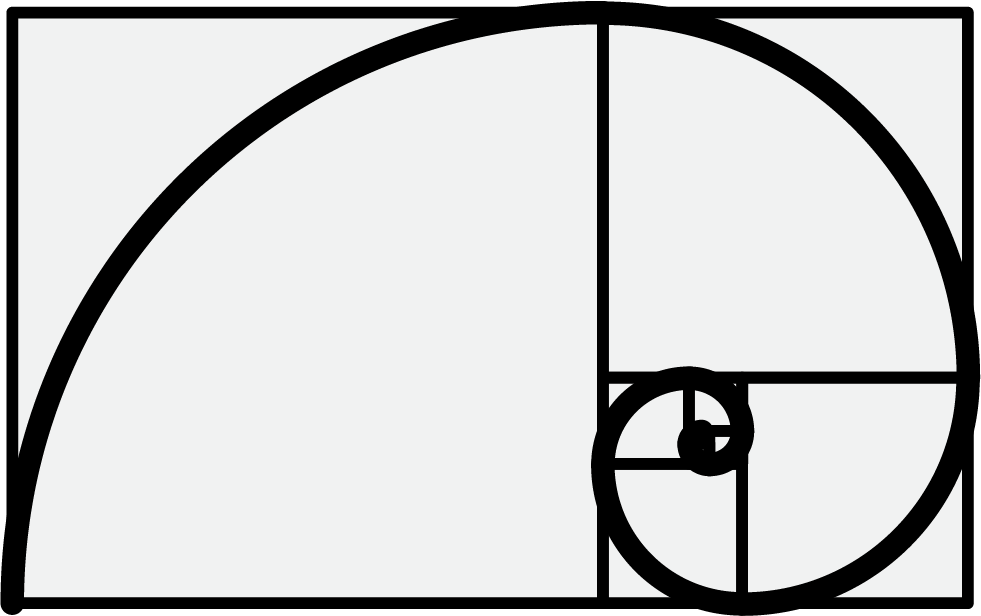
\includegraphics[height=0.75cm]{../../AAA_template_latex_settings/pwr-control_logo_doc.png}}
\lfoot{\href{http://www.pwr-control.com}{pwr-control.com}}
\cfoot{-\ \thepage\ -}
\rfoot{\textit{}}
\renewcommand{\headrulewidth}{0.4pt}
\renewcommand{\footrulewidth}{0.4pt}


\geometry{
	a4paper,
	top    = 2.5cm,
	bottom = 3.0cm,
	left   = 2.5cm,
	right  = 2.5cm
}

\hypersetup{
	colorlinks = true,
	urlcolor   = blue,
	linkcolor  = black,
	citecolor  = black
}

\pagenumbering{gobble}

\usetikzlibrary{shapes.geometric,fit,decorations.pathreplacing}

\newcommand{\ped}[1]{_{\mathrm{#1}}}
\newcommand{\code}[1]{\texttt{#1}}
\newcommand{\us}{\_\allowbreak}  % breakable underscore for long paths
\setlength{\emergencystretch}{2em}  % long code paths in justified text
\newcommand{\sat}{\operatorname{sat}}
\newcommand{\wrapop}{\operatorname{wrap}}
\renewcommand{\tabularxcolumn}[1]{>{\raggedright\arraybackslash}p{#1}}
\setlength{\emergencystretch}{3em}
\sisetup{per-mode=symbol,retain-explicit-plus}

% ---------------- document metadata (read by the title page) ----------------
\newcommand{\DocCategory}{Technical Note}
\newcommand{\DocField}{Power Electronics and Control Systems}

\newcommand{\DocTitle}{%
	{\fontsize{20}{24}\selectfont\bfseries Three-phase grid PLLs under grid faults\par}
	\vspace{14pt}
	{\fontsize{16}{23}\selectfont\bfseries dq-PLL, DDSRF-PLL and FHT-PLL of the model \code{frt\_dqpll}:\\ continuous-time models, performance on a VDE-AR-N 4110 fault,\\ criticalities and improvements\par}
}

\newcommand{\DocSubtitle}{%
	The three phase locked loops that the model \code{three\_phase\_dqPLLs\_analysis} of \code{pwr-control/modelization-and-control} runs side by side on the same grid voltage, described from the control point of view: the loop and its front ends, their transfer functions, what the simulated asymmetric fault and a set of test signals show, where each loop fails and what to change, with the DDSRF-PLL first.
}

\newcommand{\DocAuthor}{Davide Bagnara}
\newcommand{\DocRevision}{00}
\newcommand{\DocDate}{November 2026}

\newcommand{\DocAbstract}{%
	The model \code{frt\_dqpll} feeds the LCL filter of a \SI{250}{\kilo\watt} active front end from a \SI{690}{\volt} grid emulator and runs three phase locked loops on the capacitor voltage: the synchronous-frame dq-PLL, the decoupled double synchronous reference frame PLL (DDSRF-PLL) and a PLL fed by the positive sequence that two first harmonic trackers build from the $\alpha\beta$ voltages (FHT-PLL). This note writes the three loops as the blocks compute them, derives their continuous-time models (the second order phase loop with its gains, the harmonic observer of the tracker and its positive-sequence calculator, the decoupling network of the DDSRF with its poles) and compares them on the logged simulation of test 25.4 of VDE-AR-N 4110 (phase U to \num{0.25} pu, V and W to \num{0.875} pu with a \ang{21.8} shift, \SI{915}{\milli\second}) and on six test signals, with an offline re-implementation that reproduces the logged FHT-PLL within \num{4e-5} rad. The dq-PLL needs its gain scheduling in the fault and still shows a \ang{8.6} peak-to-peak ripple at \SI{100}{\hertz}; the FHT-PLL rejects the negative sequence to \ang{1.4} but its phase leads the voltage by \ang{4.15} because of two details of the C code; the DDSRF-PLL as built is fed with the negative-sequence outputs and never locks on the phase, and with the positive-sequence feed alone it locks on $-\omega$ when started from zero frequency. With the positive feed, the frequency integrator started at \num{1} pu and clamped, and the PI retuned for the low-pass filters in its loop ($k_p = 0.32$, $k_i = 8$), the DDSRF-PLL becomes the best of the three on every test except the frequency step: \ang{0.05} ripple, \ang{2.5} transient at the fault start, \ang{1.3} at its end.
}

\newcommand{\RevisionHistory}{%
	00 & November 2026 & First issue: models of the three PLLs, comparison on the logged fault and on test signals, criticalities and improvements, scripts \code{py/make\_figures.py} and \code{plotting\_results\_plls.m}. & \DocAuthor \\
}

\newcommand{\MetaLabelA}{Project Repository}
\newcommand{\MetaValueAUrl}{https://github.com/pwr-control/modelization-and-control.git}
\newcommand{\MetaValueALabel}{modelization-and-control.git (three\_phase\_dqPLLs\_analysis)}

\newcommand{\MetaLabelB}{Framework}
\newcommand{\MetaValueB}{MATLAB/Simulink, Python}

\begin{document}

% =============================================================
%  pwr-control LaTeX template - FRONTESPIZIO
%
%  Da richiamare come prima istruzione dopo \begin{document}:
%      % =============================================================
%  pwr-control LaTeX template - FRONTESPIZIO
%
%  Da richiamare come prima istruzione dopo \begin{document}:
%      % =============================================================
%  pwr-control LaTeX template - FRONTESPIZIO
%
%  Da richiamare come prima istruzione dopo \begin{document}:
%      \input{../../AAA_template_latex_settings/titlepage}
%
%  Il documento deve definire prima di \begin{document}:
%      \DocCategory   categoria del documento
%      \DocField      area tecnica
%      \DocTitle      titolo (una o due righe)
%      \DocSubtitle   sottotitolo
%      \DocAuthor     autore/i, separati da virgola
%      \DocRevision   numero di revisione corrente (es. 00)
%      \DocDate       data della revisione corrente
%      \DocAbstract   abstract
%      \RevisionHistory  righe della tabella di revisione, nel formato
%                        Rev. & Date & Description & Authors \\
%      \MetaLabelA \MetaValueAUrl \MetaValueALabel
%      \MetaLabelB \MetaValueB
% =============================================================

\providecommand{\DocCategory}{Technical Research Report}
\providecommand{\DocField}{Power Electronics and Control Systems}
\providecommand{\DocSubtitle}{}
\providecommand{\DocRevision}{00}
\providecommand{\DocAbstract}{}
\providecommand{\RevisionHistory}{%
	\DocRevision & \DocDate & First issue. & \DocAuthor \\
}

\titlepage

% ---- Intestazione centrata ----
\begin{center}
	{\Large\scshape \DocCategory}\\[8pt]
	{\large\scshape \DocField}
\end{center}

\vspace{30pt plus 4pt minus 14pt}
\noindent\rule{\linewidth}{0.8pt}

% ---- Titolo ----
\begin{center}
	\DocTitle
\end{center}

\vspace{4pt}
\noindent\rule{\linewidth}{2.2pt}

% ---- Sottotitolo ----
\begin{center}
	\begin{onehalfspace}
		{\large\itshape \DocSubtitle}
	\end{onehalfspace}
\end{center}

% ---- Authors / Revision / Date ----
\vspace{30pt plus 4pt minus 14pt}

\noindent
\begin{minipage}[t]{0.46\linewidth}
	\raggedright
	\textbf{Authors:}\\[2pt]
	\DocAuthor
\end{minipage}%
\hfill
\begin{minipage}[t]{0.22\linewidth}
	\centering
	\textbf{Revision:}\\[2pt]
	\DocRevision
\end{minipage}%
\hfill
\begin{minipage}[t]{0.30\linewidth}
	\raggedleft
	\textbf{Date:}\\[2pt]
	\DocDate
\end{minipage}

\vspace{10pt}
\noindent\rule{\linewidth}{0.8pt}

% ---- Abstract ----
\vspace{24pt plus 4pt minus 12pt}

\begin{center}
	\begin{minipage}{0.88\linewidth}
		\footnotesize
		\begin{onehalfspace}
			\textbf{Abstract:} \DocAbstract
		\end{onehalfspace}
	\end{minipage}
\end{center}

\vfill

% ---- Revision history ----
\begin{center}
	\begin{minipage}{0.96\linewidth}
		\centering
		{\footnotesize\scshape Revision history}\\[6pt]
		{\footnotesize
			\begin{tabular}{@{}cl>{\raggedright\arraybackslash}p{0.36\linewidth}>{\raggedright\arraybackslash}p{0.28\linewidth}@{}}
				\toprule
				\textbf{Rev.} & \textbf{Date} & \textbf{Description} & \textbf{Authors} \\
				\midrule
				\RevisionHistory
				\bottomrule
			\end{tabular}}
	\end{minipage}
\end{center}

\vspace{18pt plus 4pt minus 10pt}

% ---- Metadati in fondo ----
\noindent
\begin{tabular}{@{} r @{\quad} l @{}}
	\textsc{\MetaLabelA:} & {\href{\MetaValueAUrl}{\MetaValueALabel}} \\[3pt]
	\textsc{\MetaLabelB:} & {\MetaValueB}       \\[3pt]
\end{tabular}

% =============================================================
%  Fine frontespizio
% =============================================================
\newpage
\pagenumbering{arabic}
\setcounter{page}{1}

%
%  Il documento deve definire prima di \begin{document}:
%      \DocCategory   categoria del documento
%      \DocField      area tecnica
%      \DocTitle      titolo (una o due righe)
%      \DocSubtitle   sottotitolo
%      \DocAuthor     autore/i, separati da virgola
%      \DocRevision   numero di revisione corrente (es. 00)
%      \DocDate       data della revisione corrente
%      \DocAbstract   abstract
%      \RevisionHistory  righe della tabella di revisione, nel formato
%                        Rev. & Date & Description & Authors \\
%      \MetaLabelA \MetaValueAUrl \MetaValueALabel
%      \MetaLabelB \MetaValueB
% =============================================================

\providecommand{\DocCategory}{Technical Research Report}
\providecommand{\DocField}{Power Electronics and Control Systems}
\providecommand{\DocSubtitle}{}
\providecommand{\DocRevision}{00}
\providecommand{\DocAbstract}{}
\providecommand{\RevisionHistory}{%
	\DocRevision & \DocDate & First issue. & \DocAuthor \\
}

\titlepage

% ---- Intestazione centrata ----
\begin{center}
	{\Large\scshape \DocCategory}\\[8pt]
	{\large\scshape \DocField}
\end{center}

\vspace{30pt plus 4pt minus 14pt}
\noindent\rule{\linewidth}{0.8pt}

% ---- Titolo ----
\begin{center}
	\DocTitle
\end{center}

\vspace{4pt}
\noindent\rule{\linewidth}{2.2pt}

% ---- Sottotitolo ----
\begin{center}
	\begin{onehalfspace}
		{\large\itshape \DocSubtitle}
	\end{onehalfspace}
\end{center}

% ---- Authors / Revision / Date ----
\vspace{30pt plus 4pt minus 14pt}

\noindent
\begin{minipage}[t]{0.46\linewidth}
	\raggedright
	\textbf{Authors:}\\[2pt]
	\DocAuthor
\end{minipage}%
\hfill
\begin{minipage}[t]{0.22\linewidth}
	\centering
	\textbf{Revision:}\\[2pt]
	\DocRevision
\end{minipage}%
\hfill
\begin{minipage}[t]{0.30\linewidth}
	\raggedleft
	\textbf{Date:}\\[2pt]
	\DocDate
\end{minipage}

\vspace{10pt}
\noindent\rule{\linewidth}{0.8pt}

% ---- Abstract ----
\vspace{24pt plus 4pt minus 12pt}

\begin{center}
	\begin{minipage}{0.88\linewidth}
		\footnotesize
		\begin{onehalfspace}
			\textbf{Abstract:} \DocAbstract
		\end{onehalfspace}
	\end{minipage}
\end{center}

\vfill

% ---- Revision history ----
\begin{center}
	\begin{minipage}{0.96\linewidth}
		\centering
		{\footnotesize\scshape Revision history}\\[6pt]
		{\footnotesize
			\begin{tabular}{@{}cl>{\raggedright\arraybackslash}p{0.36\linewidth}>{\raggedright\arraybackslash}p{0.28\linewidth}@{}}
				\toprule
				\textbf{Rev.} & \textbf{Date} & \textbf{Description} & \textbf{Authors} \\
				\midrule
				\RevisionHistory
				\bottomrule
			\end{tabular}}
	\end{minipage}
\end{center}

\vspace{18pt plus 4pt minus 10pt}

% ---- Metadati in fondo ----
\noindent
\begin{tabular}{@{} r @{\quad} l @{}}
	\textsc{\MetaLabelA:} & {\href{\MetaValueAUrl}{\MetaValueALabel}} \\[3pt]
	\textsc{\MetaLabelB:} & {\MetaValueB}       \\[3pt]
\end{tabular}

% =============================================================
%  Fine frontespizio
% =============================================================
\newpage
\pagenumbering{arabic}
\setcounter{page}{1}

%
%  Il documento deve definire prima di \begin{document}:
%      \DocCategory   categoria del documento
%      \DocField      area tecnica
%      \DocTitle      titolo (una o due righe)
%      \DocSubtitle   sottotitolo
%      \DocAuthor     autore/i, separati da virgola
%      \DocRevision   numero di revisione corrente (es. 00)
%      \DocDate       data della revisione corrente
%      \DocAbstract   abstract
%      \RevisionHistory  righe della tabella di revisione, nel formato
%                        Rev. & Date & Description & Authors \\
%      \MetaLabelA \MetaValueAUrl \MetaValueALabel
%      \MetaLabelB \MetaValueB
% =============================================================

\providecommand{\DocCategory}{Technical Research Report}
\providecommand{\DocField}{Power Electronics and Control Systems}
\providecommand{\DocSubtitle}{}
\providecommand{\DocRevision}{00}
\providecommand{\DocAbstract}{}
\providecommand{\RevisionHistory}{%
	\DocRevision & \DocDate & First issue. & \DocAuthor \\
}

\titlepage

% ---- Intestazione centrata ----
\begin{center}
	{\Large\scshape \DocCategory}\\[8pt]
	{\large\scshape \DocField}
\end{center}

\vspace{30pt plus 4pt minus 14pt}
\noindent\rule{\linewidth}{0.8pt}

% ---- Titolo ----
\begin{center}
	\DocTitle
\end{center}

\vspace{4pt}
\noindent\rule{\linewidth}{2.2pt}

% ---- Sottotitolo ----
\begin{center}
	\begin{onehalfspace}
		{\large\itshape \DocSubtitle}
	\end{onehalfspace}
\end{center}

% ---- Authors / Revision / Date ----
\vspace{30pt plus 4pt minus 14pt}

\noindent
\begin{minipage}[t]{0.46\linewidth}
	\raggedright
	\textbf{Authors:}\\[2pt]
	\DocAuthor
\end{minipage}%
\hfill
\begin{minipage}[t]{0.22\linewidth}
	\centering
	\textbf{Revision:}\\[2pt]
	\DocRevision
\end{minipage}%
\hfill
\begin{minipage}[t]{0.30\linewidth}
	\raggedleft
	\textbf{Date:}\\[2pt]
	\DocDate
\end{minipage}

\vspace{10pt}
\noindent\rule{\linewidth}{0.8pt}

% ---- Abstract ----
\vspace{24pt plus 4pt minus 12pt}

\begin{center}
	\begin{minipage}{0.88\linewidth}
		\footnotesize
		\begin{onehalfspace}
			\textbf{Abstract:} \DocAbstract
		\end{onehalfspace}
	\end{minipage}
\end{center}

\vfill

% ---- Revision history ----
\begin{center}
	\begin{minipage}{0.96\linewidth}
		\centering
		{\footnotesize\scshape Revision history}\\[6pt]
		{\footnotesize
			\begin{tabular}{@{}cl>{\raggedright\arraybackslash}p{0.36\linewidth}>{\raggedright\arraybackslash}p{0.28\linewidth}@{}}
				\toprule
				\textbf{Rev.} & \textbf{Date} & \textbf{Description} & \textbf{Authors} \\
				\midrule
				\RevisionHistory
				\bottomrule
			\end{tabular}}
	\end{minipage}
\end{center}

\vspace{18pt plus 4pt minus 10pt}

% ---- Metadati in fondo ----
\noindent
\begin{tabular}{@{} r @{\quad} l @{}}
	\textsc{\MetaLabelA:} & {\href{\MetaValueAUrl}{\MetaValueALabel}} \\[3pt]
	\textsc{\MetaLabelB:} & {\MetaValueB}       \\[3pt]
\end{tabular}

% =============================================================
%  Fine frontespizio
% =============================================================
\newpage
\pagenumbering{arabic}
\setcounter{page}{1}


\tableofcontents
\listoffigures
\listoftables
\newpage

\begin{onehalfspace}

% =============================================================
\section*{Nomenclature}
\addcontentsline{toc}{section}{Nomenclature}
\label{sec:nomenclature}

\begingroup
\rowcolors{2}{tableShade}{white}
\begin{longtable}{@{} >{\raggedright\arraybackslash}p{0.22\linewidth} p{0.74\linewidth} @{}}
	\toprule
	\textbf{Symbol} & \textbf{Meaning} \\
	\midrule
	\endfirsthead
	\toprule
	\textbf{Symbol} & \textbf{Meaning} \\
	\midrule
	\endhead
	\bottomrule
	\endfoot
	\bottomrule
	\endlastfoot
	PLL & phase locked loop: the estimate of the angle $\theta$ and of the pulsation $\omega$ of the grid voltage \\
	dq-PLL, SRF-PLL & PLL in the synchronous reference frame (the $\xi\eta$ frame of the model) \\
	DDSRF-PLL & PLL on the decoupled double synchronous reference frame (positive and negative frame) \\
	FHT, FHT-PLL & first harmonic tracker (library C code) and the PLL fed by the positive sequence built from two trackers \\
	abc, $\alpha\beta$, $\xi\eta$ & phase quantities, stationary two-axis frame (amplitude-invariant Clarke transform), rotating frame \\
	pos, neg & positive and negative sequence; the positive frame turns by $+\theta$, the negative frame by $-\theta$ \\
	pu & per unit of the peak phase voltage of the converter class (\SI{690}{\volt}: \SI{563}{\volt} peak) \\
	$\theta\ped{g}$, $\theta$ & angle of the grid voltage (positive sequence) and its estimate by the PLL \\
	$\omega\ped{n}$, $f\ped{0}$, $\omega_0$ & nominal grid pulsation $2\pi f\ped{0}$, $f\ped{0} = \SI{50}{\hertz}$; $\omega_0$ is the same number as the resonance of the trackers \\
	$\omega\ped{pu}$ & estimated grid pulsation in pu of $\omega\ped{n}$ \\
	$t\ped{s}$ & control period, \SI{125}{\micro\second} (\SI{4}{\kilo\hertz} PWM, double update) \\
	$u$, $\hat u$, $\hat v$ & grid voltage (pu), its estimate by a tracker and the quadrature estimate ($\hat v = \hat{\dot u}/\omega_0$) \\
	$u\ped{sr}$ & output of the positive-sequence calculator of the FHT-PLL (minus the positive sequence) \\
	$u\ped{pos}$, $u\ped{neg}$ & decoupled positive and negative sequence of the DDSRF block, as $\xi\eta$ pairs \\
	$V\ped{norm}$ & normalization of the phase detector, $1/\sqrt{\max(\alpha^2+\beta^2,\,0.02)}$ \\
	$e$ & input of the loop PI: the normalized $\eta$ component of the positive sequence (the phase error for small errors) \\
	$k\ped{p}$, $k\ped{i}$ & proportional and integral gain of the loop PI (\code{pll\_p}, \code{pll\_i1} of \code{ctrl\_afe\_setup}) \\
	$\omega\ped{c}$, $\zeta$ & natural frequency and damping of the phase loop; $\omega\ped{x}$ its crossover, PM its phase margin \\
	$T(s)$, $L(s)$ & closed loop (phase from the detector input) and open loop of the phase loop \\
	$H_1$, $H_2$, $D$ & transfer functions of the tracker, $\hat u / u$ and $\hat{\dot u} / u$, and their denominator \\
	$l_1$, $l_2$, $\delta$ & observer gains and damping of the tracker; $L\ped{d} = [l_1\ l_2]$ the discrete gains of the C code \\
	$G(\omega)$ & complex gain of a positive-sequence calculator on a component $e^{j\omega t}$ of $\alpha + j\beta$ ($\omega < 0$: negative sequence) \\
	$F(s)$, $\omega\ped{f}$, $\tau$ & low-pass filter of the DDSRF, $\omega\ped{f}/(s+\omega\ped{f})$, $\omega\ped{f} = 1/\tau$ \\
	$A\ped{d}$, $L\ped{dso}$ & matrices of the double-integrator observer of stage B \\
	$\sat$, $\wrapop$ & saturation between two limits; angle wrapped to $(-\pi, \pi]$: $-\pi + \bmod(u + 3\pi,\, 2\pi)$ \\
	FRT, LVRT & fault ride-through, low-voltage ride-through; \code{frt\_active} is the flag of the FRT detector \\
	$z$ & variable of the $z$ transform, $z = e^{j\omega t\ped{s}}$ on the unit circle \\
\end{longtable}
\endgroup
\addtocounter{table}{-1}

% =============================================================
\section{Introduction}
\label{sec:intro}

The model \code{frt\_dqpll.slx} of \code{foundations\us of\us power\us electronics/\allowbreak three\us phase\us dqPLLs\us analysis} \cite{model_repo} is a test bench for grid synchronization: a \SI{1}{\mega\watt}, \SI{690}{\volt} grid emulator with its Dyn11 transformer feeds the LCL filter of a \SI{250}{\kilo\watt} active front end whose converter side is open, and the AFE control (\SI{125}{\micro\second}) runs four phase locked loops on the normalized capacitor voltage: the dq-PLL in Simulink, the same loop as a C caller, the DDSRF-PLL and the FHT-PLL. One of them (by default the FHT-PLL) gives the angle and the frequency to the grid-support blocks of the library \code{afe\_uvw\_ctrl} \cite{library_repo, note_uvw}. The grid emulator applies test 25.4 of VDE-AR-N 4110 \cite{vde4110} in its asymmetric variant: phase U drops to \num{0.25} pu, phases V and W to \num{0.875} pu with a shift of \ang{21.8} each, a type D dip with a positive sequence of \num{0.625} pu and a negative sequence of \num{0.375} pu, from \SI{0.75}{\second} for \SI{915}{\milli\second}.

This note describes the three Simulink loops (the C caller is a copy of the dq-PLL and is not treated) from the control point of view:
\begin{itemize}[nosep]
	\item Section~\ref{sec:loop} writes the loop that the three PLLs share (stage B of the blocks: PI, phase integrator, double integrator observer), its continuous-time model and its discrete poles;
	\item Section~\ref{sec:frontends} writes the three front ends (stage A): the synchronous frame of the dq-PLL, the first harmonic tracker and the positive-sequence calculator of the FHT-PLL, the decoupling network of the DDSRF-PLL, each with its transfer functions and with the implementation details of the blocks and of the C code that change them;
	\item Section~\ref{sec:logged} compares the loops on the logged simulation of the fault and Section~\ref{sec:synth} on six test signals (phase jump, frequency step, balanced sag, unbalance, harmonics, DC offset);
	\item Section~\ref{sec:crit} lists the criticalities of each loop and what to change, with the DDSRF-PLL first, and Section~\ref{sec:summary} gives the recommendation.
\end{itemize}

\paragraph{How the results were obtained.} The simulation logs the outputs of the FHT-PLL only (the Variant Source removes the other branches from the compiled model), so the comparison runs the three algorithms offline on the logged capacitor voltage \code{ugd\_abc\_grid\_sim}, step by step as the blocks and the C code compute them: control period, one-step delays, clamps, resets. The offline FHT-PLL reproduces the logged phase \code{phase\_grid\_fhtsr\_dqpll\_sim} within \num{3.9e-5} rad (\num{1e-5} rad after the first \SI{20}{\milli\second}) and the logged tracker signals within \num{1e-6} pu, which validates the common parts (Clarke transform, normalization, stage B, observer) and the tracker; the dq-PLL and the DDSRF-PLL are transcribed from the diagrams with the same elements. Two scripts do this: \code{py/make\_figures.py} with \code{py/pll\_models.py} in this folder (Python, every figure and number of the note) and \code{plotting\_results\_plls.m} in the model folder (MATLAB, the same runs and figures after a simulation, Section~\ref{sec:files}). The reference angle is the angle of the logged voltage itself: a linear fit of the $\alpha\beta$ angle before the fault, which gives \SI{49.990}{\hertz} (the emulator runs \num{0.02}~\% below nominal, the logged FHT-PLL frequency says the same) and holds through the fault because a type D dip does not move the positive sequence (one-period DFT: \num{0.6254} pu at \ang{0.00} during the fault).

% =============================================================
\section{The loop shared by the three PLLs}
\label{sec:loop}

Every PLL of the model is split in two subsystems (Figure~\ref{fig:structure}): stage A turns the three phase voltages into the $\xi\eta$ components of the positive sequence in the frame of the estimated angle, and stage B closes the loop on the $\eta$ component. Stage B is the same block in the three loops, with the gains of the class \code{ctrl\_afe\_setup}: \code{pll\_p} $= 1$, \code{pll\_i1} $= 80$ (the DDSRF and FHT loops copy them as \code{pll\_p\_ddsrt}, \code{pll\_p\_fht}, \ldots).

\begin{figure}[H]
	\centering
	\begin{tikzpicture}[font=\scriptsize, >=Latex,
		blk/.style={draw, thick, rounded corners=2pt, fill=orange!15, minimum width=2.6cm, minimum height=0.9cm, align=center},
		sm/.style={draw, thick, rounded corners=2pt, fill=gray!12, minimum width=1.6cm, minimum height=0.7cm, align=center}]
		\node[blk] (a) at (0,0) {stage A\\abc $\to$ pos. sequence $\xi\eta$};
		\node[sm] (n) at (3.2,0) {$\times V\ped{norm}$};
		\node[sm] (pi) at (5.6,0) {$k\ped{p} + k\ped{i}/s$};
		\node[sm] (int) at (8.0,0) {$\omega\ped{n}/s$, wrap};
		\node[sm] (obs) at (8.0,-1.5) {DI observer};
		\draw[->] (-1.8,0) node[left] {$u\ped{abc}$} -- (a);
		\draw[->] (a) -- node[above] {$u\ped{pos,\eta}$} (n);
		\draw[->] (n) -- node[above] {$e$} (pi);
		\draw[->] (pi) -- node[above] {$\omega\ped{pu}$} (int);
		\draw[->] (int) -- (10.3,0) node[right] {$\theta$};
		\draw[->] (9.3,0) |- (obs);
		\draw[->] (obs) -- (10.3,-1.5) node[right] {$\omega\ped{pu}$ (output)};
		\draw[->] (9.0,0) -- (9.0,1.0) -| node[pos=0.25, above] {$\theta$ (one step late)} (a);
	\end{tikzpicture}
	\caption{Structure of the three PLLs: stage A (the front end, different in the three blocks) and stage B (the same loop). The normalization $V\ped{norm}$ is computed in stage A from the $\alpha\beta$ voltage that reaches the rotation.}
	\label{fig:structure}
\end{figure}

\subsection{Stage B as the block computes it}
\label{sec:stageB}

With $\eta$ the second output of stage A, $V\ped{norm} = 1/\sqrt{\max(\alpha^2 + \beta^2,\, 0.02)}$ and $s\ped{B} = \pm 1$ the sign in front of the PI ($+1$ in the dq-PLL, $-1$ in the FHT-PLL and in the DDSRF-PLL, where a Gain block of $-1$ sits before the PI), step $k$ of stage B is
\begin{align}
	e[k] &= s\ped{B}\, \eta[k]\, V\ped{norm}[k], \\
	i[k] &= \sat\big(i[k-1] + k\ped{i} t\ped{s}\, e[k]\big), \qquad \omega\ped{pu}[k] = k\ped{p}\, e[k] + i[k], \label{eq:pi} \\
	\theta[k] &= \wrapop\big(\theta[k-1] + t\ped{s}\, \omega\ped{n}\, \omega\ped{pu}[k]\big), \label{eq:theta}
\end{align}
and the outputs of the block at step $k$ are $\theta[k-1]$ (a Unit Delay) and the frequency estimate of the double integrator observer. The saturation of the integrator is $\pm 2$ pu in the dq-PLL and absent in the other two. The integrator starts at zero: every PLL of the model starts from zero frequency. The angle that stage A uses at step $k$ is the same $\theta[k-1]$, so in steady state, with a constant grid frequency, the output of the block at step $k$ is the angle of the voltage sampled at step $k$: the one-step delay of the structure costs no phase (the PI drives $\eta$ to zero on the delayed angle, and the integrator holds the frequency).

The double integrator observer estimates the frequency from the wrapped phase with the states $x = [\hat\theta,\ \hat\omega]^T$:
\begin{equation}
	x[k+1] = A\ped{d}\, x[k] + L\ped{dso}\, \wrapop\big(\theta[k-1] - \wrapop(\hat\theta[k])\big), \qquad A\ped{d} = \begin{bmatrix} 1 & t\ped{s} \\ 0 & 1 \end{bmatrix},
\end{equation}
with the frequency output $\omega\ped{pu,out}[k] = \hat\omega[k]/\omega\ped{n}$ and $L\ped{dso} = [0.1839,\ 44.78]^T$ from Ackermann's formula at the poles $e^{-\omega\ped{n} t\ped{s}}$ and $e^{-4\omega\ped{n} t\ped{s}}$ (continuous poles $-\omega\ped{n}$ and $-4\omega\ped{n}$, \SI{3.2}{\milli\second} and \SI{0.8}{\milli\second}). The frequency output therefore follows the loop frequency $\omega\ped{pu}$ of \eqref{eq:pi} with about \SI{4}{\milli\second} of delay and without its proportional kick; it is this output that the rest of the control reads (\code{omega\_grid\_pll\_pu}) and that the figures of this note show.

\subsection{Continuous-time model and gains}
\label{sec:loopmodel}

For small errors $\eta\, V\ped{norm} \approx \sin(\theta\ped{g} - \theta) \approx \theta\ped{g} - \theta$ (the normalization removes the voltage amplitude), and \eqref{eq:pi}--\eqref{eq:theta} are the second order loop
\begin{equation}
	\dot\theta = \omega\ped{n}\Big(k\ped{p}\, e + k\ped{i} \int e\Big), \quad e = \theta\ped{g} - \theta + d
	\qquad\Longrightarrow\qquad
	T(s) = \frac{\theta}{\theta\ped{g} + d} = \frac{\omega\ped{n}(k\ped{p} s + k\ped{i})}{s^2 + \omega\ped{n} k\ped{p}\, s + \omega\ped{n} k\ped{i}},
	\label{eq:T}
\end{equation}
where $d$ collects everything that enters the detector besides the phase error: the negative sequence at $2\omega$, the harmonics $6\omega$, $12\omega$, \ldots, a DC offset at $\omega$. The natural frequency is $\omega\ped{c} = \sqrt{\omega\ped{n} k\ped{i}}$ and the damping $\zeta = \omega\ped{n} k\ped{p} / (2\omega\ped{c})$. The loop is of type 2 for the angle: zero steady-state error for a frequency step. Table~\ref{tab:gains} gives the numbers of the gain sets that appear in this note; the open loop $L(s) = \omega\ped{n}(k\ped{p} s + k\ped{i})/s^2$ crosses at $\omega\ped{x} \approx \omega\ped{n} k\ped{p}$ ($L \approx \omega\ped{n} k\ped{p}/s$ well above the PI corner $k\ped{i}/k\ped{p}$), so with $k\ped{p} = 1$ the loop crosses at \SI{324}{\radian\per\second} (\SI{52}{\hertz}) and attenuates the \SI{100}{\hertz} term of the detector only to $|T(j2\omega\ped{n})| = 0.475$ (Figure~\ref{fig:loops}, left). The last two columns anticipate Section~\ref{sec:ddsrf}: with the low-pass filter $F(s) = \omega\ped{f}/(s+\omega\ped{f})$ of the DDSRF in the loop, the same gains lose half of their phase margin.

\begin{table}[H]
	\centering
	\caption{Gain sets of the phase loop \eqref{eq:T}: the gains of the model, the fault gains of the dq-PLL (\code{pll\_p\_frt}), the alternative fault set of the README of the model and the set proposed for the DDSRF-PLL. Crossover $\omega\ped{x}$ and phase margin without and with the low-pass filter $\omega\ped{f} = \omega\ped{n}$ of the DDSRF in the loop.}
	\label{tab:gains}
	\footnotesize
	\setlength{\tabcolsep}{4pt}
	\rowcolors{3}{tableShade}{white}
	\begin{tabular}{@{} l c c c c c c c c c c @{}}
		\toprule
		gain set & $k\ped{p}$ & $k\ped{i}$ & $\omega\ped{c}$ & $\zeta$ & $|T(j2\omega\ped{n})|$ & $|T(j6\omega\ped{n})|$ & \multicolumn{2}{c}{without LPF} & \multicolumn{2}{c@{}}{with LPF} \\
		 & & & [rad/s] (Hz) & & & & $\omega\ped{x}$ [rad/s] & PM & $\omega\ped{x}$ [rad/s] & PM \\
		\midrule
		model & 1 & 80 & 159 (25.2) & 0.99 & 0.475 & 0.166 & 324 & \ang{76} & 255 & \ang{33} \\
		dq-PLL in the fault & 0.2 & 80 & 159 (25.2) & 0.20 & 0.126 & 0.034 & 165 & \ang{22} & 155 & \ang{-5} \\
		alternative fault set & 0.2 & 3.2 & 32 (5.0) & 0.99 & 0.100 & 0.033 & 65 & \ang{76} & 64 & \ang{64} \\
		proposed, DDSRF-PLL & 0.32 & 8 & 50 (8.0) & 1.00 & 0.159 & 0.053 & 103 & \ang{76} & 99 & \ang{58} \\
		\bottomrule
	\end{tabular}
	\rowcolors{1}{white}{white}
\end{table}

\begin{figure}[H]
	\centering
	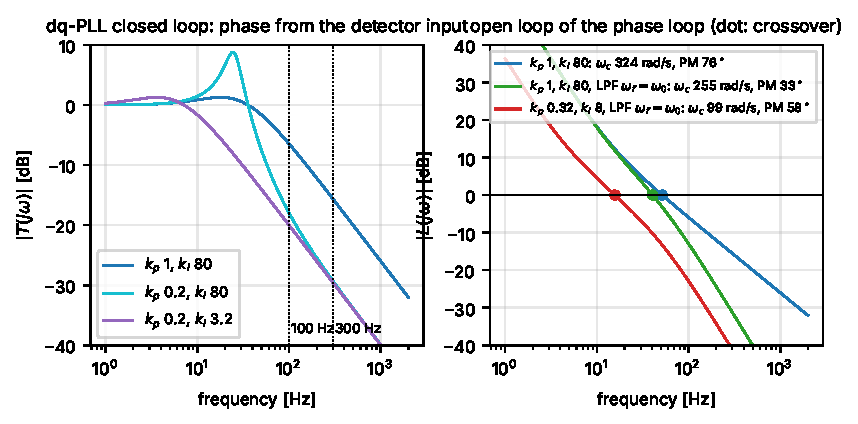
\includegraphics[width=\textwidth]{figures/pll_loops.pdf}
	\caption{Left: closed loop $|T(j\omega)|$ of the phase loop for the three gain sets of the dq-PLL; the dotted lines mark the \SI{100}{\hertz} of the negative sequence and the \SI{300}{\hertz} of the 5th and 7th harmonics. Right: open loop of the same PI with and without the low-pass filter of the DDSRF-PLL in the loop; the dots mark the crossover.}
	\label{fig:loops}
\end{figure}

\paragraph{Discrete loop.} With the forward Euler integrators of \eqref{eq:pi}--\eqref{eq:theta} and the one-step delay of the angle, the poles of the discrete loop are $z = 0.9794,\ 0.9809$ for the normal gains, i.e.\ $s = -166,\ -154$ \si{\radian\per\second} against the continuous $-157 \pm 21j$: at \SI{125}{\micro\second} the discretization changes nothing that matters, for any of the gain sets (\code{pll\_design} of the model init prints the same numbers). The fault gains give the poles $-31 \pm 156j$ \si{\radian\per\second}, a damping of \num{0.20}: a phase jump rings at \SI{25}{\hertz} for about \SI{150}{\milli\second}.

% =============================================================
\section{The three front ends}
\label{sec:frontends}

\subsection{dq-PLL: the synchronous frame}
\label{sec:dq}

Stage A of the dq-PLL is the Clarke transform (amplitude invariant, $\alpha = \tfrac{2}{3}(u\ped{a} - \tfrac{1}{2}u\ped{b} - \tfrac{1}{2}u\ped{c})$, $\beta = (u\ped{b} - u\ped{c})/\sqrt{3}$), the normalization and the rotation by $-\theta$ (chart \code{alphabeta2xieta\_pos}):
\begin{equation}
	\xi = \alpha\cos\theta + \beta\sin\theta, \qquad \eta = -\alpha\sin\theta + \beta\cos\theta,
	\label{eq:rotpos}
\end{equation}
so that for $\alpha + j\beta = V e^{j\theta\ped{g}}$ the detector gives $\eta\, V\ped{norm} = \sin(\theta\ped{g} - \theta)$. Nothing filters the voltage: a negative sequence $V\ped{n} e^{-j\theta\ped{g}}$ gives $\eta \ni -V\ped{n}\sin(\theta\ped{g}+\theta) \approx -V\ped{n}\sin 2\theta\ped{g}$, a term at $2\omega$ that the loop attenuates only by $|T(j2\omega\ped{n})|$; the 5th and 7th harmonics give a term at $6\omega$, a DC offset of the measurement a term at $\omega$. The normalization uses the total $\alpha\beta$ magnitude $|V\ped{p} + V\ped{n} e^{-j2\theta\ped{g}}|$, which during an unbalance oscillates at $2\omega$ too and modulates the loop gain between $1/(V\ped{p}+V\ped{n})$ and $1/(V\ped{p}-V\ped{n})$.

The only countermeasure of the block is the scheduled proportional gain: the Switch of \code{scheduled-p-gain} takes $k\ped{p} = $ \code{pll\_p\_frt} $= 0.2$ while the FRT detector of the library (\code{frt\_vde4110}, on the averaged sequences) holds \code{frt\_active}, and keeps $k\ped{i} = 80$. This reduces the ripple gain from \num{0.475} to \num{0.126} (Table~\ref{tab:gains}) at the price of the damping: $\zeta$ drops from \num{0.99} to \num{0.20}, and the recovery of the normal gain at the end of the fault happens with the integrator loaded by the ripple.

\subsection{FHT-PLL: first harmonic trackers and the positive-sequence calculator}
\label{sec:fht}

\paragraph{The tracker.} The first harmonic tracker of the library (\code{first\_harmonic\_tracker.c}, parameters \code{fht\_grid} of \code{ctrl\_afe\_setup}) is a Luenberger observer of a damped harmonic oscillator at $\omega_0 = \omega\ped{n}$, with the state $x_1$ the estimate $\hat u$ of its input and $x_2$ the estimate of its derivative:
\begin{equation}
	\dot x_1 = x_2 + l_1 (u - x_1), \qquad \dot x_2 = -\omega_0^2\, x_1 - \delta\omega_0\, x_2 + l_2 (u - x_1), \qquad \hat u = x_1, \quad \hat v = x_2/\omega_0,
	\label{eq:fht}
\end{equation}
with $\delta = 0.05$ and the gains placed at the poles $-\omega_0$ and $-4\omega_0$: the characteristic polynomial $s^2 + (l_1 + \delta\omega_0)s + l_1\delta\omega_0 + \omega_0^2 + l_2 = (s+\omega_0)(s+4\omega_0)$ gives $l_1 = 4.95\,\omega_0 = \SI{1555}{\per\second}$ and $l_2 = 2.7525\,\omega_0^2$. The transfer functions from the input are
\begin{align}
	H_1(s) &= \frac{\hat u}{u} = \frac{l_1 s + l_1\delta\omega_0 + l_2}{D(s)}, \qquad
	H_2(s) = \frac{\hat{\dot u}}{u} = \frac{l_2 s - l_1\omega_0^2}{D(s)}, \notag \\
	D(s) &= s^2 + (l_1+\delta\omega_0)s + l_1\delta\omega_0 + \omega_0^2 + l_2.
	\label{eq:H12}
\end{align}
At $s = j\omega_0$ the term $\omega_0^2$ of $D$ cancels $s^2$ and $H_1(j\omega_0) = 0.993\angle\ang{-0.25}$: a unity-gain band-pass whose width is set by the observer poles, $l_1 \approx 5\omega_0$, i.e.\ about \SI{250}{\hertz}. This is the point to keep in mind: the tracker converges in \SI{4}{\milli\second} (\num{5}~\% error after \SI{3.9}{\milli\second} from a cold start) because it is wide, and for the same reason it passes the 5th and 7th harmonics with a gain of \num{0.35} and \num{0.40} and a DC offset with \num{0.72} (Table~\ref{tab:fht}). It is a fast estimator of the fundamental, not a selective filter.

\paragraph{The positive-sequence calculator.} Stage A of the FHT-PLL (Figure~\ref{fig:fht}) runs one tracker on $\alpha$ and one on $\beta$ and combines the in-phase and quadrature estimates as
\begin{equation}
	u\ped{sr,\alpha} = -\tfrac{1}{2}\big(\hat u_\alpha + \hat v_\beta\big), \qquad u\ped{sr,\beta} = -\tfrac{1}{2}\big(\hat u_\beta - \hat v_\alpha\big),
	\qquad\text{i.e.}\qquad u\ped{sr} = -\tfrac{1}{2}\big(\hat u - j\hat v\big) \ \text{ in complex form},
	\label{eq:psc}
\end{equation}
which is the classic positive-sequence calculator built on a quadrature signal generator: for a positive sequence $e^{j\omega_0 t}$ the quadrature is $\hat v = j\hat u$ and \eqref{eq:psc} gives $-\hat u$, for a negative sequence $e^{-j\omega_0 t}$ it is $\hat v = -j\hat u$ and the output is zero. The minus sign is compensated by the Gain $-1$ in front of the PI of stage B ($s\ped{B} = -1$), and the normalization uses $|u\ped{sr}|$, which is the positive sequence only. For a component $e^{j\omega t}$ of $\alpha + j\beta$ (with $\omega < 0$ for a negative sequence) the output is $-G(\omega)\, e^{j\omega t}$ with
\begin{align}
	G(\omega) &= \tfrac{1}{2}\Big(H_1(j\omega) - j\,\frac{H_2(j\omega)}{\omega_0}\Big), \notag \\
	G(\omega_0) &= \frac{(l_1\delta\omega_0 + 2 l_2) + 2j\, l_1\omega_0}{2 D(j\omega_0)} = 0.982\angle\ang{+0.80},
	\qquad
	|G(-\omega_0)| = \frac{l_1\delta\omega_0}{2|D(j\omega_0)|} = 0.021 .
	\label{eq:G}
\end{align}
The damping $\delta$ is the only reason why the calculator is not exact at $\omega_0$: with $\delta = 0$ the quadrature state is the exact derivative in steady state, $G(\omega_0) = 1$ and $G(-\omega_0) = 0$. With $\delta = 0.05$ the positive sequence leads the input by \ang{0.8} and \num{2.1}~\% of the negative sequence leaks into the output.

\begin{figure}[H]
	\centering
	\begin{tikzpicture}[font=\scriptsize, >=Latex,
		blk/.style={draw, thick, rounded corners=2pt, fill=orange!15, minimum width=1.9cm, minimum height=0.8cm, align=center},
		sm/.style={draw, thick, rounded corners=2pt, fill=gray!12, minimum width=1.4cm, minimum height=0.7cm, align=center}]
		\node[sm] (cl) at (0,0) {Clarke};
		\node[blk] (fa) at (2.6,0.8) {FHT on $\alpha$\\$\hat u_\alpha,\ \hat v_\alpha$};
		\node[blk] (fb) at (2.6,-0.8) {FHT on $\beta$\\$\hat u_\beta,\ \hat v_\beta$};
		\node[blk, minimum width=3.4cm] (ps) at (6.0,0) {$u\ped{sr} = -\tfrac12(\hat u - j\hat v)$\\positive-sequence calculator};
		\node[sm] (rot) at (9.2,0) {rotation $-\theta$};
		\draw[->] (-1.6,0) node[left] {$u\ped{abc}$} -- (cl);
		\draw[->] (cl) |- (fa); \draw[->] (cl) |- (fb);
		\draw[->] (fa) -| (ps.north west) ; \draw[->] (fb) -| (ps.south west);
		\draw[->] (ps) -- (rot);
		\draw[->] (rot) -- (11.0,0) node[right] {$\xi,\ \eta$};
		\draw[->] (9.2,-1.4) node[below] {$\theta$ from stage B} -- (rot);
		\draw[->] (ps.north) -- (6.0,1.6) node[above] {$V\ped{norm} = 1/|u\ped{sr}|$};
	\end{tikzpicture}
	\caption{Stage A of the FHT-PLL. The two trackers are two instances of the library C code with the parameters \code{fht\_grid} (resonance $\omega_0 = \omega\ped{n}$, $\delta = 0.05$, gains $L\ped{d}$), held in reset for the first \SI{12.5}{\milli\second}.}
	\label{fig:fht}
\end{figure}

\paragraph{The discrete implementation.} The C code integrates \eqref{eq:fht} with the second order Taylor matrix of the oscillator ($A\ped{d} = I + A t\ped{s} + \tfrac12 A^2 t\ped{s}^2$, Section 7 of the README of the model) and with the gains $L\ped{d} = [0.1819,\ 29.59]$ designed with Ackermann's formula on the forward Euler matrix $I + A t\ped{s}$ at the poles $e^{-\omega_0 t\ped{s}}$, $e^{-4\omega_0 t\ped{s}}$. Two details of \code{first\_harmonic\_tracker\_process} change the response at the fundamental:
\begin{enumerate}[nosep]
	\item the innovation is computed with the output stored at the \emph{previous} call, $u[k] - \hat u[k-1]$, not with the current predicted state: $x[k+1] = A\ped{d}\, x[k] + L\ped{d}\,(u[k] - x_1[k-1])$. The observer has three poles instead of two, $z = 0.962,\ 0.805,\ 0.230$ ($s = -312,\ -1733,\ -11\,776$ \si{\radian\per\second}) instead of the designed $z = 0.961,\ 0.854$ ($-320,\ -1264$): still stable and fast, but the output $\hat u[k] = x_1[k]$ now \emph{leads} a \SI{50}{\hertz} input by \ang{1.96} (gain \num{0.992}) where the designed observer lags by \ang{0.28};
	\item the quadrature output is the state \emph{after} the update, $\hat v[k] = x_2[k+1]/\omega_0$, one step ahead of $\hat u[k] = x_1[k]$. At \SI{50}{\hertz} one step is \ang{2.25}.
\end{enumerate}
Table~\ref{tab:fht} and Figure~\ref{fig:fhtfe} give the resulting gain of the calculator for the components of interest, next to the continuous model and to two variants that change only the code: the same observer with consistent states ($\hat u = x_1[k]$, $\hat v = x_2[k]/\omega_0$ and the innovation on the current state), and the same with $\delta = 0$ (gains recomputed for the same poles). The leak of the negative sequence doubles in the code as it is (\num{3.9}~\% instead of \num{2.1}~\%: the quadrature of a negative sequence is one step off) and the positive sequence leads the sampled voltage by \ang{4.15}. The lead depends on the frequency, about \ang{0.8} per hertz, because the tracker is tuned at the fixed $\omega_0 = \omega\ped{n}$ and does not follow the PLL frequency.

\begin{table}[H]
	\centering
	\caption{Gain $|G|$ and angle of the positive-sequence calculator of the FHT-PLL on a component of $\alpha+j\beta$ at the given frequency (negative frequency: negative sequence). Continuous model \eqref{eq:G}; library C code as it is (delayed innovation, quadrature one step ahead); same observer with consistent states; consistent states and $\delta = 0$.}
	\label{tab:fht}
	\rowcolors{2}{tableShade}{white}
	\begin{tabular}{@{} l c c c c @{}}
		\toprule
		component & continuous & C code as is & consistent states & consistent, $\delta = 0$ \\
		\midrule
		fundamental, \SI{+50}{\hertz} & 0.982 / \ang{0.8} & 0.981 / \ang{4.1} & 0.981 / \ang{0.8} & 1.000 / \ang{0.0} \\
		negative sequence, \SI{-50}{\hertz} & 0.021 & 0.039 & 0.021 & 0.000 \\
		\SI{+49}{\hertz} & 0.983 / \ang{1.6} & 0.982 / \ang{4.9} & 0.982 / \ang{1.7} & 1.001 / \ang{0.9} \\
		\SI{+51}{\hertz} & 0.981 / \ang{0.0} & 0.980 / \ang{3.4} & 0.980 / \ang{0.0} & 0.999 / \ang{-0.8} \\
		\SI{-51}{\hertz} & 0.018 & 0.034 & 0.019 & 0.010 \\
		DC & 0.724 & 0.716 & 0.716 & 0.722 \\
		2nd, \SI{+100}{\hertz} & 0.856 & 0.892 & 0.861 & 0.881 \\
		5th, \SI{-250}{\hertz} & 0.345 & 0.350 & 0.350 & 0.362 \\
		7th, \SI{+350}{\hertz} & 0.398 & 0.520 & 0.405 & 0.416 \\
		11th, \SI{-550}{\hertz} & 0.219 & 0.212 & 0.224 & 0.231 \\
		13th, \SI{+650}{\hertz} & 0.224 & 0.325 & 0.229 & 0.236 \\
		\bottomrule
	\end{tabular}
	\rowcolors{1}{white}{white}
\end{table}

\begin{figure}[H]
	\centering
	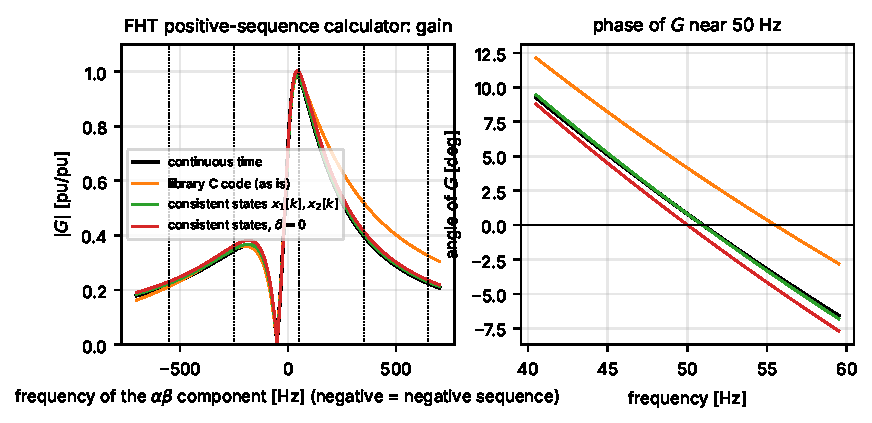
\includegraphics[width=\textwidth]{figures/fht_frontend.pdf}
	\caption{Positive-sequence calculator of the FHT-PLL: gain on a component of $\alpha + j\beta$ against its (signed) frequency, dotted lines at the harmonics of interest (left), and the phase of the output around the fundamental (right), for the continuous model, the C code as it is and the two variants of Table~\ref{tab:fht}.}
	\label{fig:fhtfe}
\end{figure}

\subsection{DDSRF-PLL: the decoupling network}
\label{sec:ddsrf}

Stage A of the DDSRF-PLL (Figure~\ref{fig:ddsrf}) pre-filters each phase voltage with a tracker (three instances of the C code, output $\hat u$ only), takes the Clarke transform of the three estimates, computes $V\ped{norm}$ from it and feeds the block \code{sequences/ddsrf}: the rotations by $-\theta$ (positive frame, \eqref{eq:rotpos}) and by $+\theta$ (negative frame, chart \code{alphabeta2xieta\_neg}: $\xi = \alpha\cos\theta - \beta\sin\theta$, $\eta = \alpha\sin\theta + \beta\cos\theta$), four library low-pass filters with $\tau = $ \code{tau\_ddsrf} $= 1/\omega\ped{n}$ and the cross decoupling of \cite{rodriguez2007}. In complex form, with $u = \alpha + j\beta$, $p = u\ped{pos,\xi} + j u\ped{pos,\eta}$, $n = u\ped{neg,\xi} + j u\ped{neg,\eta}$ and $F(s) = \omega\ped{f}/(s + \omega\ped{f})$, $\omega\ped{f} = 1/\tau$:
\begin{equation}
	p = F(s)\Big[u\, e^{-j\theta} - n\, e^{-j2\theta}\Big], \qquad
	n = F(s)\Big[u\, e^{+j\theta} - p\, e^{+j2\theta}\Big].
	\label{eq:ddsrf}
\end{equation}
In the positive frame the positive sequence is a constant and the negative sequence turns at $-2\omega$; the network subtracts from each frame the \emph{filtered} estimate of the other sequence rotated into it. The two properties of \eqref{eq:ddsrf} that the comparison needs are:
\begin{itemize}[nosep]
	\item \textbf{the steady state is exact.} With $\theta = \omega t$, $u = V\ped{p} e^{j\omega t} + V\ped{n} e^{-j\omega t}$, writing $p = P_0 + P_2 e^{-j2\omega t}$, $n = N_0 + N_2 e^{j2\omega t}$ and using $F(0) = 1$ gives $P_0 = V\ped{p} - N_2$, $N_2 = F(j2\omega)(V\ped{p} - P_0)$, hence $P_0 = V\ped{p}$, $P_2 = 0$, $N_0 = V\ped{n}$, $N_2 = 0$: the decoupled outputs carry no $2\omega$ term at all, whatever $\omega\ped{f}$. This is why the ripple of the DDSRF-PLL in Sections~\ref{sec:logged} and \ref{sec:synth} is two orders of magnitude below the one of the dq-PLL, and why $\omega\ped{f}$ is a choice about dynamics only;
	\item \textbf{the dynamics.} A perturbation $\tilde p$ at the complex frequency $s$ in the positive frame reaches the negative frame at $s + j2\omega$ and comes back: $\tilde p = F(s)\,F(s+j2\omega)\,\tilde p$, so the sequence estimation error decays with the roots of $1 - F(s)F(s + j2\omega) = 0$,
	\begin{equation}
		s = -(\omega\ped{f} + j\omega) \pm \sqrt{\omega\ped{f}^2 - \omega^2} .
		\label{eq:ddpoles}
	\end{equation}
	For $\omega\ped{f} \le \omega$ both roots have the real part $-\omega\ped{f}$; for $\omega\ped{f} > \omega$ they split and one of them slows down towards $-\omega^2/(2\omega\ped{f})$. The fastest decay is at $\omega\ped{f} = \omega$, a double root at $-\omega - j\omega$ (\SI{3.2}{\milli\second}): the model's choice $\tau = 1/\omega\ped{n}$ is the optimum of \eqref{eq:ddpoles} (Table~\ref{tab:ddpoles}, Figure~\ref{fig:ddpoles}). The price is the attenuation of what the filters are also asked to remove from the frames: the 6th harmonic passes with $|F(j6\omega)| = 0.164$ and a DC offset, which appears at $\omega$ in both frames, with \num{0.707}.
\end{itemize}

\begin{table}[H]
	\centering
	\caption{Roots \eqref{eq:ddpoles} of the decoupling network and attenuation of the low-pass filter for different corner frequencies; $\omega\ped{f} = \omega_0$ is the value of the model.}
	\label{tab:ddpoles}
	\rowcolors{3}{tableShade}{white}
	\begin{tabular}{@{} l c c c c c c @{}}
		\toprule
		$\omega\ped{f}$ & $\tau$ & root 1 & root 2 & slowest time & $|F(j2\omega_0)|$ & $|F(j6\omega_0)|$ \\
		 & [ms] & [rad/s] & [rad/s] & constant [ms] & & \\
		\midrule
		$\omega_0/2$ & 6.37 & $-157 - 42j$ & $-157 - 586j$ & 6.37 & 0.243 & 0.083 \\
		$\omega_0/\sqrt{2}$ & 4.50 & $-222 - 92j$ & $-222 - 536j$ & 4.50 & 0.333 & 0.117 \\
		$\omega_0$ (model) & 3.18 & $-314 - 314j$ & $-314 - 314j$ & 3.18 & 0.447 & 0.164 \\
		$1.5\,\omega_0$ & 2.12 & $-120 - 314j$ & $-822 - 314j$ & 8.33 & 0.600 & 0.243 \\
		$2\,\omega_0$ & 1.59 & $-84 - 314j$ & $-1172 - 314j$ & 11.9 & 0.707 & 0.316 \\
		\bottomrule
	\end{tabular}
	\rowcolors{1}{white}{white}
\end{table}

\begin{figure}[H]
	\centering
	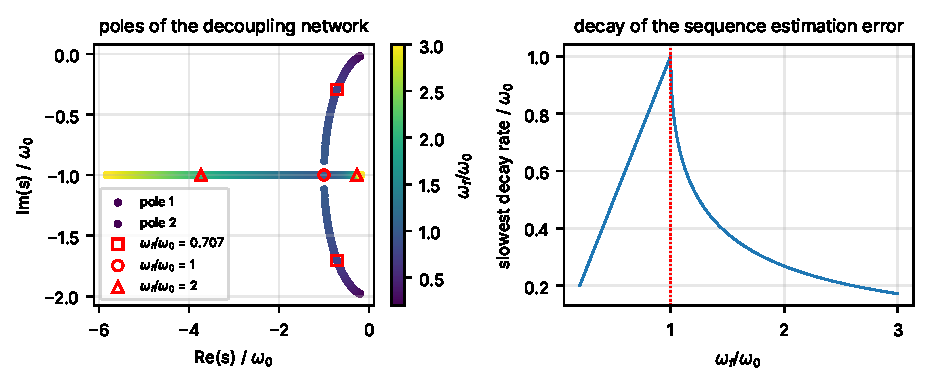
\includegraphics[width=\textwidth]{figures/ddsrf_poles.pdf}
	\caption{Roots of the decoupling network \eqref{eq:ddpoles} as $\omega\ped{f}/\omega_0$ goes from \num{0.2} to \num{3} (left; the markers are $1/\sqrt2$, $1$ and $2$) and the slowest decay rate (right): the fastest separation of the sequences is at $\omega\ped{f} = \omega_0$.}
	\label{fig:ddpoles}
\end{figure}

\begin{figure}[H]
	\centering
	\resizebox{\textwidth}{!}{%
	\begin{tikzpicture}[font=\scriptsize, >=Latex,
		blk/.style={draw, thick, rounded corners=2pt, fill=orange!15, minimum width=2.0cm, minimum height=0.8cm, align=center},
		sm/.style={draw, thick, rounded corners=2pt, fill=gray!12, minimum width=1.3cm, minimum height=0.7cm, align=center},
		sum/.style={draw, thick, circle, inner sep=1pt, minimum size=0.45cm}]
		\node[blk] (pre) at (0,0) {3 FHT\\(one per phase)};
		\node[sm] (cl) at (2.4,0) {Clarke};
		\node[sm] (rp) at (4.6,1.1) {rot.\ $-\theta$};
		\node[sm] (rn) at (4.6,-1.1) {rot.\ $+\theta$};
		\node[sum] (sp) at (6.4,1.1) {$-$};
		\node[sum] (sn) at (6.4,-1.1) {$-$};
		\node[sm] (fp) at (8.0,1.1) {$F(s)$};
		\node[sm] (fn) at (8.0,-1.1) {$F(s)$};
		\node[sm] (dp) at (8.0,0.0) {rot.\ $+2\theta$};
		\node[sm] (dn) at (10.2,0.0) {rot.\ $-2\theta$};
		\draw[->] (-1.8,0) node[left] {$u\ped{abc}$} -- (pre);
		\draw[->] (pre) -- node[above] {$\hat u\ped{abc}$} (cl);
		\draw[->] (cl) |- (rp); \draw[->] (cl) |- (rn);
		\draw[->] (rp) -- (sp); \draw[->] (rn) -- (sn);
		\draw[->] (sp) -- (fp); \draw[->] (sn) -- (fn);
		\draw[->] (fp) -- (11.6,1.1) node[right] {$u\ped{pos}$ (outputs 1, 2)};
		\draw[->] (fn) -- (11.6,-1.1) node[right] {$u\ped{neg}$ (outputs 3, 4)};
		\draw[->] (9.2,1.1) -- (9.2,0.55) -| (dn.north);
		\draw[->] (dn.south) |- (6.4,-0.5) -- (sn);
		\draw[->] (9.2,-1.1) -- (9.2,-0.55) -| (dp.south);
		\draw[->] (dp.north) |- (6.4,0.5) -- (sp);
		\draw[->] (cl.north) -- (2.4,1.9) node[above] {$V\ped{norm}$ from $\hat u_{\alpha\beta}$};
		\node[draw, dashed, rounded corners=2pt, fit=(rp) (rn) (sp) (sn) (fp) (fn) (dp) (dn), inner sep=5pt, label={[font=\scriptsize]below:\code{sequences/ddsrf}}] {};
	\end{tikzpicture}}
	\caption{Stage A of the DDSRF-PLL. Stage B of the model is wired to the outputs 3 and 4 (the negative sequence) through the Gain $-1$; the loop of \cite{rodriguez2007} and of the corrected variants of this note takes the outputs 1 and 2.}
	\label{fig:ddsrf}
\end{figure}

\paragraph{The loop with the filter in it.} The decoupled $\eta$ of the positive sequence is $F(s)$ applied to the phase error (for small errors and no unbalance), so the open loop of the DDSRF-PLL is $F(s)\, L(s)$. With the gains of the model the crossover moves from \SI{324}{} to \SI{255}{\radian\per\second} and the phase margin from \ang{76} to \ang{33} (Table~\ref{tab:gains}, Figure~\ref{fig:loops} right): the step responses of Section~\ref{sec:synth} ring and settle in \SI{165}{\milli\second} where the dq-PLL settles in \SI{35}{\milli\second}. The fault gains of the dq-PLL would be unstable here (PM \ang{-5}). A PI chosen for this loop is in the last row of the table: $k\ped{p} = 0.32$ gives $\omega\ped{x} \approx \omega\ped{n} k\ped{p} = \SI{100}{\radian\per\second}$ (\SI{16}{\hertz}), $k\ped{i} = 8$ puts the PI corner at \SI{25}{\radian\per\second}, a quarter of the crossover, and the margin is \ang{58} with the filter.

\paragraph{The wiring of the model.} In \code{frt\_dqpll.slx} the outports of the subsystem \code{sequences} are named \code{u\_grid\_pos\_xi}, \code{u\_grid\_pos\_eta} but are connected to the outputs 3 and 4 of the \code{ddsrf} block, the \emph{negative} sequence, and stage B multiplies them by $-1$ before the PI. The loop therefore drives $u\ped{neg,\eta}$ to zero. For a negative sequence $V\ped{n} e^{-j(\omega t - \varphi)}$ the negative-frame $\eta$ is $V\ped{n}\sin(\theta - \omega t + \varphi)$, so the loop locks $\theta$ on the mirrored angle of the negative sequence, $\omega t - \varphi$: during the fault it is a negative-sequence PLL. With a balanced grid the negative outputs are zero whatever $\theta$ is and the loop has no phase information: the frequency still converges towards $\omega$ through the $2\omega$ terms that an angle error leaks into the negative frame before the decoupling settles, but the phase is arbitrary (Section~\ref{sec:logged}: \ang{-40} to \ang{-52} before the fault, drifting). The intended loop, the one of \cite{rodriguez2007}, takes the outputs 1 and 2 with $s\ped{B} = +1$; the note calls it ``positive feed''.

% =============================================================
\section{Performance on the simulated fault}
\label{sec:logged}

The logged run is \SI{2.25}{\second} long, with the fault from \SI{0.75}{\second} to \SI{1.665}{\second} (Figure~\ref{fig:voltage}): the capacitor voltage shows the \SI{20}{\milli\second} ramps of the fault generator, the LCL ringing at \SI{1284}{\hertz} at every step (README of the model) and the two sequences of the type D dip, \num{0.625} and \num{0.375} pu, with the positive sequence at the same angle as before the fault. The seven variants of Table~\ref{tab:logged} are run on this voltage; Figures~\ref{fig:asbuilt} to \ref{fig:loggedddsrf} show them. ``Lock'' is the last time before the fault at which the phase error (minus its steady-state offset) exceeds \ang{1}; ``settle'' the same after the fault start and after its end; ``ripple'' the peak-to-peak phase error between \SI{1.2}{} and \SI{1.65}{\second}. The flag \code{frt\_active} is not logged: the scheduled gain of the dq-PLL is applied on the fault window itself (the detector of the library reacts within a few milliseconds).

\begin{figure}[H]
	\centering
	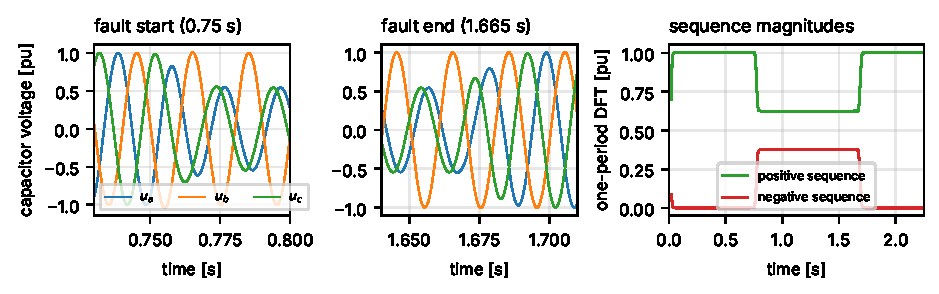
\includegraphics[width=\textwidth]{figures/logged_voltage.pdf}
	\caption{Logged capacitor voltage (pu) at the start and at the end of the fault, and the sequence magnitudes from a one-period DFT on the reference angle.}
	\label{fig:voltage}
\end{figure}

\begin{table}[H]
	\centering
	\setlength{\tabcolsep}{4pt}
	\caption{The PLL variants on the logged fault. Offset: mean phase error against the voltage angle before the fault; lock from zero frequency; peak and settling (to \ang{1}) at the fault start and end; peak-to-peak ripple of the phase and of the frequency output inside the fault. The DDSRF-PLL with the positive feed and zero start locks on $-\omega$ (its ``ripple'' of \ang{360} is the error wrapping). $^{*}$Improved: positive feed, integrator started at \num{1} pu and clamped to $[0.5,\ 1.5]$, $k\ped{p} = 0.32$, $k\ped{i} = 8$.}
	\label{tab:logged}
	\footnotesize
	\setlength{\tabcolsep}{3pt}
	\rowcolors{3}{tableShade}{white}
	\begin{tabular}{@{} l c c c c c c c c @{}}
		\toprule
		variant & offset & lock & fault start & settle & ripple & $\omega$ ripple & fault end & settle \\
		 & [deg] & [ms] & peak [deg] & [ms] & [deg pp] & [pu pp] & peak [deg] & [ms] \\
		\midrule
		dq-PLL, $k\ped{p}$ 1 fixed & 0.00 & 37 & 19.5 & 915 & 33.6 & 0.460 & 15.4 & 21 \\
		dq-PLL, scheduled $k\ped{p}$ (model) & 0.00 & 37 & 4.9 & 915 & 8.6 & 0.120 & 16.2 & 23 \\
		FHT-PLL & 4.15 & 59 & 1.8 & 23 & 1.38 & 0.019 & 1.9 & 16 \\
		DDSRF-PLL as built (neg. feed) & $-48.7$ & no & 228 & no & 0.10 & 0.001 & 172 & no \\
		DDSRF-PLL, pos. feed, zero start & $-\omega$ lock & no & 180 & no & 360 & 0.001 & 180 & no \\
		DDSRF-PLL, pos. feed, init 1 pu & 1.96 & 158 & 3.9 & 26 & 0.33 & 0.004 & 3.5 & 24 \\
		DDSRF-PLL improved$^{*}$ & 1.96 & 107 & 2.5 & 36 & 0.05 & 0.000 & 1.3 & 32 \\
		\bottomrule
	\end{tabular}
	\rowcolors{1}{white}{white}
\end{table}

\begin{figure}[H]
	\centering
	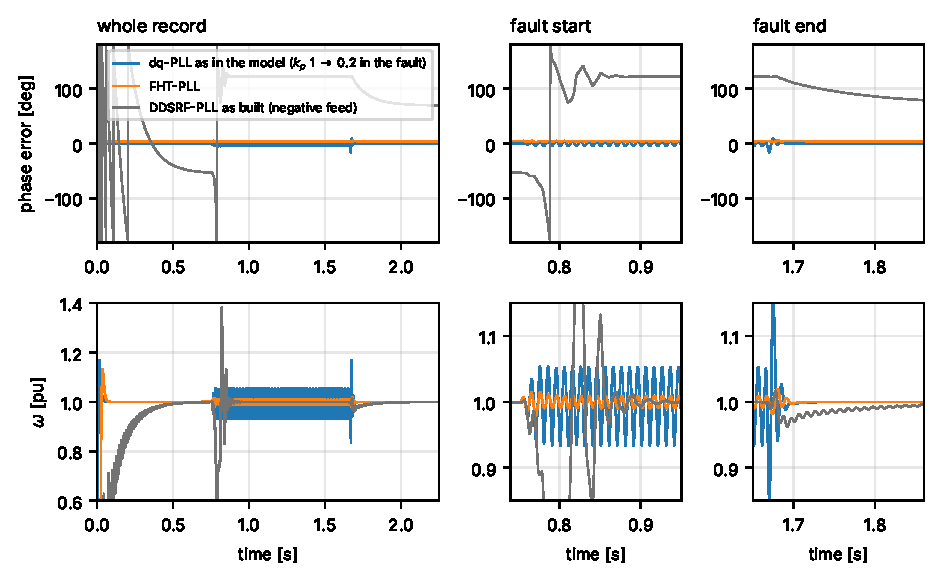
\includegraphics[width=\textwidth]{figures/logged_as_built.pdf}
	\caption{The three PLLs as they are in the model, on the logged voltage: phase error against the voltage angle (top) and frequency output (bottom), whole record and zooms at the fault start and end. The DDSRF-PLL as built never locks on the phase; the dq-PLL carries the \SI{100}{\hertz} ripple through the whole fault.}
	\label{fig:asbuilt}
\end{figure}

\begin{figure}[htb]
	\centering
	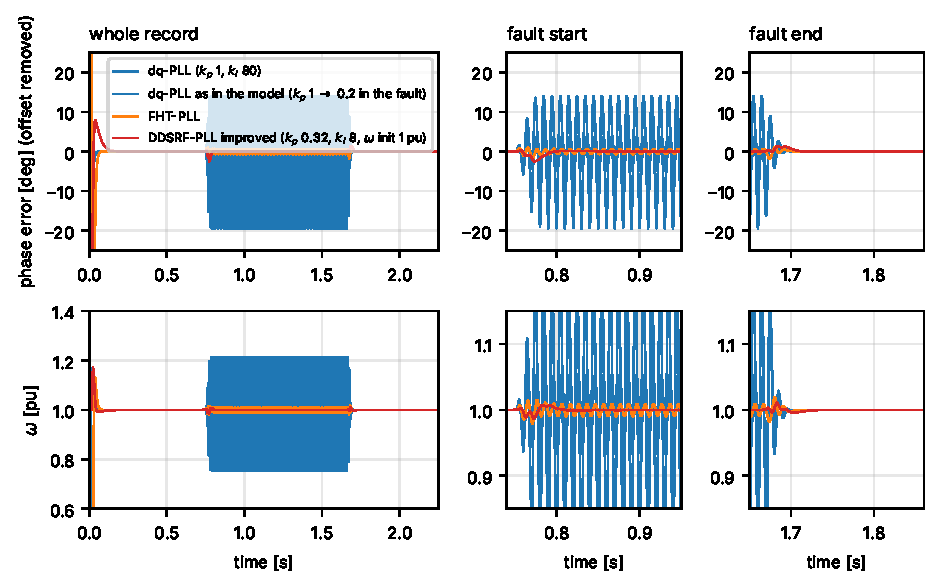
\includegraphics[width=\textwidth]{figures/logged_compare.pdf}
	\caption{Same run, steady-state offsets removed: the dq-PLL with constant and with scheduled gain, the FHT-PLL and the improved DDSRF-PLL.}
	\label{fig:compare}
\end{figure}

\begin{figure}[htb]
	\centering
	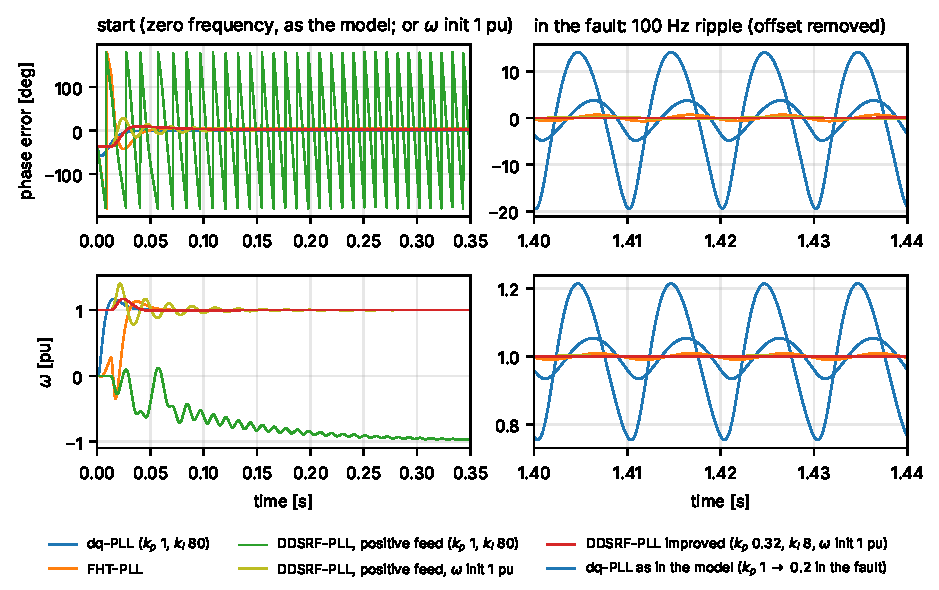
\includegraphics[width=\textwidth]{figures/logged_startup_ripple.pdf}
	\caption{Left: start from zero frequency as in the model (dq-PLL, FHT-PLL, DDSRF-PLL with the positive feed) and with the integrator initialized at \num{1} pu (two DDSRF variants); the positive feed started from zero converges to $\omega\ped{pu} = -1$. Right: \SI{40}{\milli\second} inside the fault, the \SI{100}{\hertz} ripple of the five variants.}
	\label{fig:startup}
\end{figure}

\begin{figure}[htb]
	\centering
	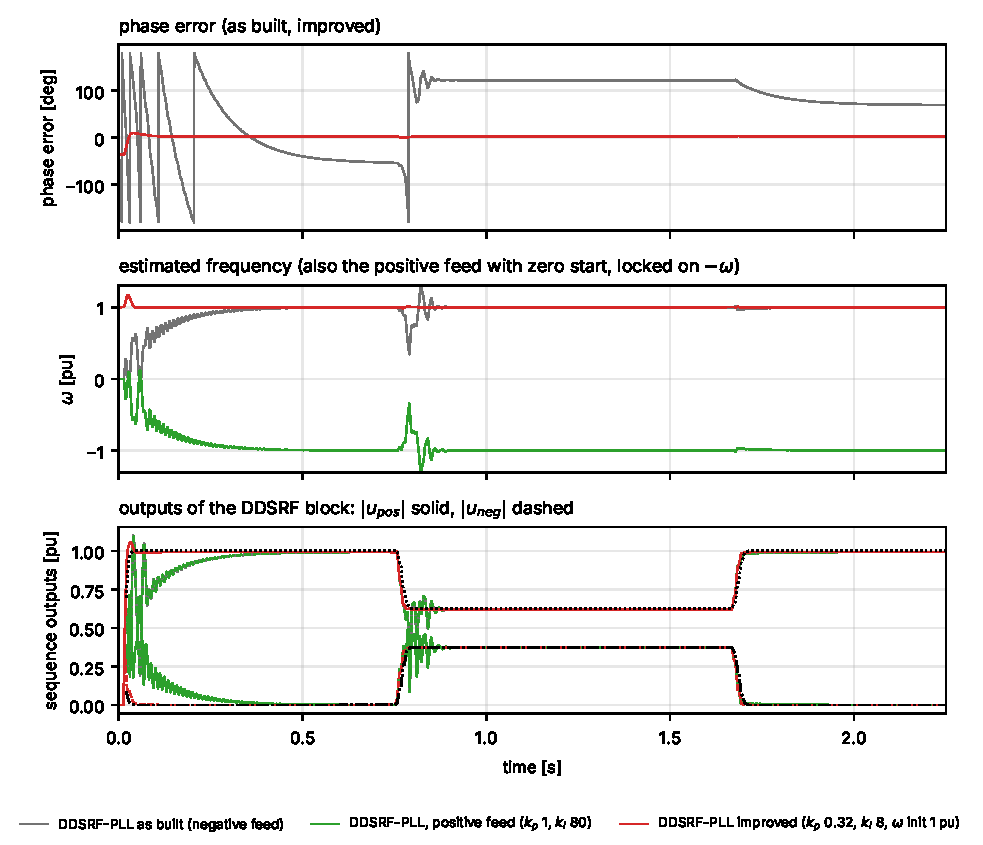
\includegraphics[width=0.95\textwidth]{figures/logged_ddsrf.pdf}
	\caption{DDSRF-PLL variants on the logged voltage: phase error of the loop as built and of the improved loop (top), frequency output of the three variants (middle), magnitude of the two sequence outputs of the \code{ddsrf} block against the true sequences (bottom). As built, the block separates the sequences correctly only during the fault, when the loop is locked on the negative sequence.}
	\label{fig:loggedddsrf}
\end{figure}

\paragraph{dq-PLL.} With the normal gains the \num{0.375} pu negative sequence gives a \ang{33.6} peak-to-peak ripple at \SI{100}{\hertz} on the phase and \num{0.46} pu on the frequency output: linear prediction $2 \cdot (V\ped{n}/V\ped{p}) \cdot |T(j2\omega\ped{n})| = 2 \cdot 0.6 \cdot 0.475$ \si{\radian} $= \ang{32.7}$, the rest is the modulation of the normalization. The scheduled gain brings the ripple to \ang{8.6} (prediction \ang{8.7}) and the frequency ripple to \num{0.12} pu, still enough to disturb the FRT state machine and the reactive current references that read \code{omega\_grid\_pll\_pu} and \code{phase\_grid\_pll}. The transient at the fault start is small with the fault gains (\ang{4.9}) but the recovery at the fault end, when the normal gain comes back with the integrator loaded by the ripple, peaks at \ang{16.2}: the same as without scheduling.

\paragraph{FHT-PLL.} Lock in \SI{59}{\milli\second} from zero frequency (the trackers are held in reset for \SI{12.5}{\milli\second}), \ang{1.8} at the fault start, \ang{1.9} at its end, \SI{23}{} and \SI{16}{\milli\second} to settle, a ripple of \ang{1.38} peak-to-peak: the leak of \num{3.9}~\% of Table~\ref{tab:fht} on \num{0.375} pu of negative sequence is \num{0.0147} pu against the \num{0.613} pu of positive sequence that the calculator outputs, \ang{1.37} peak-to-peak on the angle of $u\ped{sr}$ (measured on the logged $u\ped{sr}$: \ang{2.81}, with the normalization and the DFT bias of a finite record), attenuated by $|T(j2\omega\ped{n})| = 0.475$. The phase of the FHT-PLL leads the sampled voltage by \ang{4.15} all the time (\ang{4.154} on the logged phase, \ang{4.154} on the logged $u\ped{sr}$, \ang{1.958} on the logged tracker outputs: the numbers of Table~\ref{tab:fht}).

\paragraph{DDSRF-PLL as built.} The frequency converges (\num{0.9966} pu before the fault, \num{0.9998} inside it) but the phase does not: \ang{-40} at \SI{0.5}{\second}, \ang{-52} at \SI{0.7}{\second}, then a lock at \ang{+122} inside the fault, which is the mirrored angle of the negative sequence, and a drift after the fault. The block output $|u\ped{neg}|$ follows the true negative sequence inside the fault (\num{0.372} pu) because the loop is locked on it. The positive feed alone, started from zero frequency as every PLL of the model, converges to $\omega\ped{pu} = -0.9989$ with $|u\ped{neg}| = 0.992$ pu: the network explains a positive sequence seen from a frame turning backwards as a negative sequence, with no $\eta$ error left, so the lock on $-\omega$ is a stable equilibrium of the DDSRF-PLL that the dq-PLL and the FHT-PLL do not have (their detector keeps a $2\omega$ term there that pulls the loop out). With the integrator started at \num{1} pu the positive feed locks in \SI{158}{\milli\second} (the margin of \ang{33} shows in the slow, ringing acquisition) and goes through the fault with a \ang{3.9} transient and a \ang{0.33} ripple. The improved variant (positive feed, integrator at \num{1} pu clamped to $[0.5,\ 1.5]$, $k\ped{p} = 0.32$, $k\ped{i} = 8$) is the best line of Table~\ref{tab:logged}: \ang{2.5} at the fault start, \ang{1.3} at its end, \ang{0.05} of ripple, \num{4e-4} pu on the frequency output; its offset of \ang{1.96} is the lead of the three pre-filter trackers (Section~\ref{sec:fht}).

% =============================================================
\section{Performance on test signals}
\label{sec:synth}

The six tests of Table~\ref{tab:synth} are ideal three-phase sets at \SI{125}{\micro\second}, with every loop started locked at \num{1} pu, the event at \SI{0.4}{\second} and, for the dips, its end at \SI{0.8}{\second}. Five variants are compared: the dq-PLL with the normal gains and with the fault gains held all the time, the FHT-PLL, the DDSRF-PLL with the positive feed and the gains of the model, and the improved DDSRF-PLL. The figures~\ref{fig:synthsteps} and \ref{fig:synthdist} show the phase error with its steady-state offset removed and the frequency output.

\begin{table}[H]
	\centering
	\setlength{\tabcolsep}{3.5pt}
	\setlength{\LTcapwidth}{\textwidth}
	\caption{Test signals: peak phase error [deg] / time to settle within \ang{0.5} [ms] / peak-to-peak ripple in steady state [deg]. ``400'' means not settled within the \SI{400}{\milli\second} of the event (a permanent ripple). Harmonics: 5th \num{5}~\% negative, 7th \num{3}~\% positive, 11th \num{2}~\% negative, 13th \num{1.5}~\% positive. DC offset: \num{2}~\% of the peak voltage on phase a.}
	\label{tab:synth}
	\footnotesize
	\setlength{\tabcolsep}{4pt}
	\rowcolors{2}{tableShade}{white}
	\begin{tabular}{@{} l c c c @{}}
		\toprule
		variant & phase jump \ang{30} & frequency step \SI{+1}{\hertz} & sag to \num{0.3} pu \\
		\midrule
		dq-PLL, $k\ped{p}$ 1, $k\ped{i}$ 80 & 30 / 35 / 0 & 0.84 / 15 / 0 & 0 / 0 / 0 \\
		dq-PLL, fault gains ($k\ped{p}$ 0.2) & 30 / 124 / 0.01 & 1.72 / 36 / 0 & 0 / 0 / 0 \\
		FHT-PLL & 30 / 37 / 0 & 1.61 / 400 / 0 & 8.2 / 17 / 0 \\
		DDSRF-PLL, pos. feed, model gains & 30 / 165 / 0.13 & 1.69 / 54 / 0 & 42.4 / 191 / 0.26 \\
		DDSRF-PLL improved & 30 / 107 / 0 & 3.37 / 103 / 0 & 11.6 / 30 / 0 \\
		\midrule
		\rowcolor{white} variant & type D dip & harmonics & DC offset \num{2}~\% \\
		\midrule
		dq-PLL, $k\ped{p}$ 1, $k\ped{i}$ 80 & 21.4 / 400 / 33.5 & 0.32 / 0 / 0.39 & 0.67 / 400 / 1.28 \\
		dq-PLL, fault gains ($k\ped{p}$ 0.2) & 12.8 / 400 / 8.6 & 0.12 / 0 / 0.08 & 0.59 / 23 / 0.65 \\
		FHT-PLL & 9.5 / 400 / 1.34 & 0.26 / 0 / 0.42 & 0.49 / 0 / 0.94 \\
		DDSRF-PLL, pos. feed, model gains & 11.7 / 161 / 0.04 & 0.18 / 0 / 0.08 & 2.91 / 400 / 5.1 \\
		DDSRF-PLL improved & 3.1 / 28 / 0 & 0.07 / 0 / 0.03 & 0.37 / 0 / 0.49 \\
		\bottomrule
	\end{tabular}
	\rowcolors{1}{white}{white}
\end{table}

\begin{figure}[H]
	\centering
	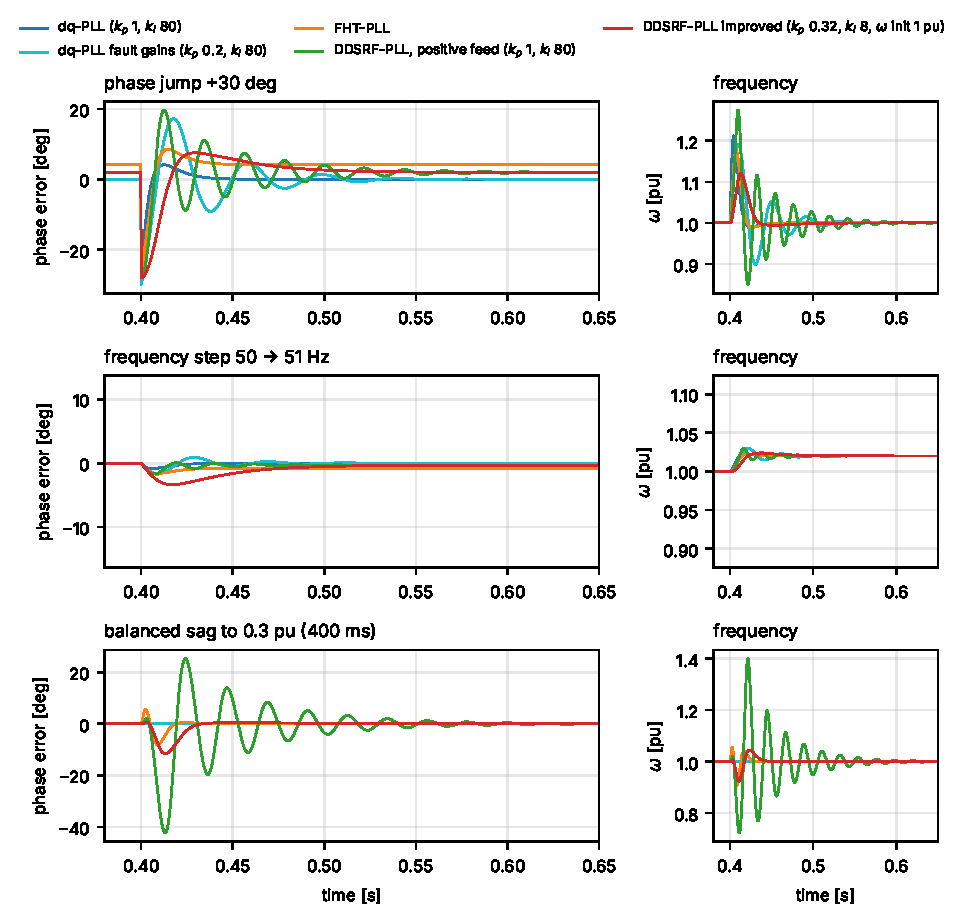
\includegraphics[width=\textwidth]{figures/synth_steps.pdf}
	\caption{Test signals, steps: phase jump of \ang{30}, frequency step from \SI{50}{} to \SI{51}{\hertz}, balanced sag to \num{0.3} pu. Phase error with the steady-state offset removed (left) and frequency output (right).}
	\label{fig:synthsteps}
\end{figure}

\begin{figure}[H]
	\centering
	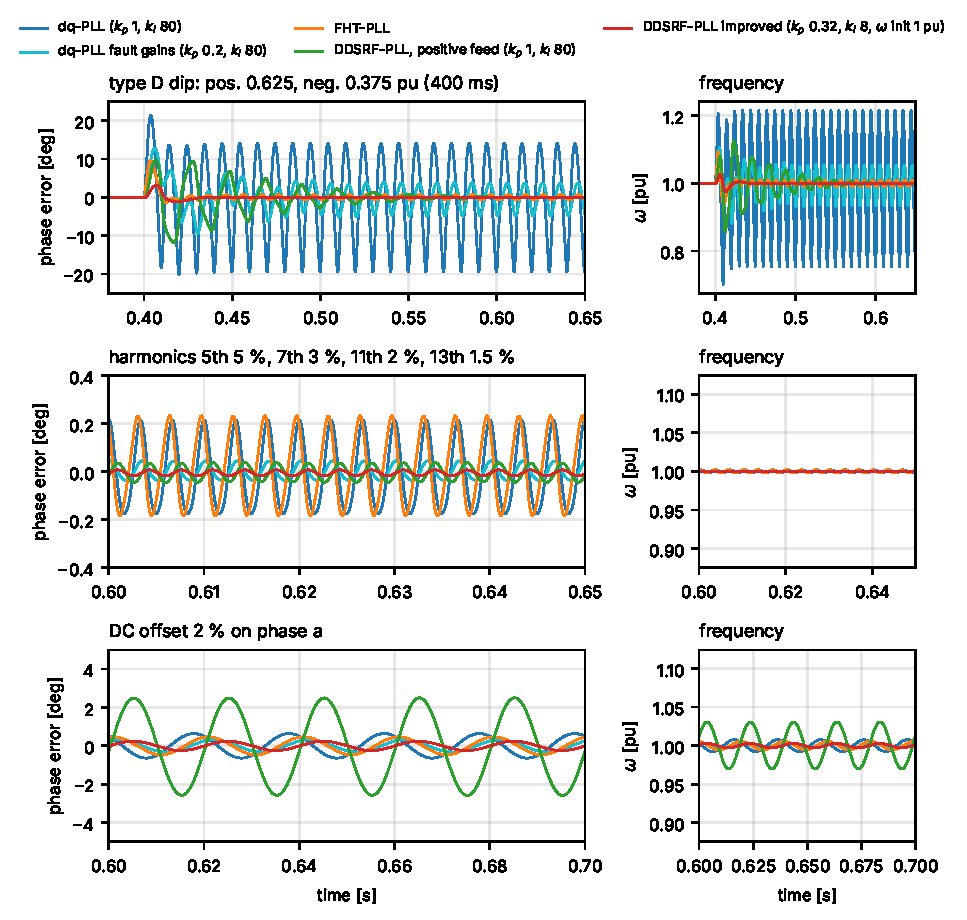
\includegraphics[width=\textwidth]{figures/synth_disturbances.pdf}
	\caption{Test signals, disturbances: type D dip (positive \num{0.625}, negative \num{0.375} pu), harmonics, DC offset of \num{2}~\% on phase a. Phase error with the steady-state offset removed (left, zoomed in time for the two steady-state tests) and frequency output (right).}
	\label{fig:synthdist}
\end{figure}

\begin{itemize}
	\item \textbf{Phase jump.} All loops peak at the \ang{30} of the jump; the dq-PLL and the FHT-PLL settle in \SI{35}{\milli\second} (the damping \num{0.99} of the loop), the fault gains in \SI{124}{\milli\second} (damping \num{0.20}), the DDSRF-PLL in \SI{165}{\milli\second} with the model gains (margin \ang{33}) and in \SI{107}{\milli\second} with the proposed ones.
	\item \textbf{Frequency step.} A \num{2}~\% step gives \ang{0.8} on the dq-PLL and \ang{1.5} to \ang{1.7} on the others; the slower improved DDSRF-PLL peaks at \ang{3.4}. The FHT-PLL never settles within \ang{0.5}: its steady-state lead changes by \ang{0.8} between \SI{50}{} and \SI{51}{\hertz} (Table~\ref{tab:fht}), a frequency-dependent bias that the type 2 loop cannot remove because it is in the front end.
	\item \textbf{Balanced sag.} The dq-PLL does not see it (the normalization is exact). The FHT-PLL shows the transient of its trackers, \ang{8.2} for \SI{17}{\milli\second}. The DDSRF-PLL swings to \ang{42} with the model gains and to \ang{129} without the pre-filters (not in the table): at the step the positive-frame filter still holds the old \num{1} pu, the decoupling injects the difference, rotated at $2\omega$, into the negative frame and back into the positive $\eta$, and the normalization by the new \num{0.3} pu amplifies the false error by \num{3.3}. The improved gains bring it to \ang{11.6}, the pre-filters help because they smooth the step. A deeper sag makes this worse: it is the first criticality of the DDSRF-PLL on balanced faults.
	\item \textbf{Type D dip.} The ripple separates the three structures: \ang{33.5} for the dq-PLL (\ang{8.6} with the fault gains, the number of the logged run), \ang{1.34} for the FHT-PLL (the leak of its calculator), below \ang{0.05} for the DDSRF-PLL (exact steady state). The transient at the dip is \ang{3.1} for the improved DDSRF-PLL against \ang{9.5} to \ang{21} for the others.
	\item \textbf{Harmonics.} The dq-PLL and the FHT-PLL are the same (\ang{0.4} peak-to-peak): the tracker gives no selectivity at the 5th and 7th. The low-pass filters of the DDSRF-PLL add their attenuation (\ang{0.08}, \ang{0.03} with the lower gains).
	\item \textbf{DC offset.} \num{2}~\% on one phase gives \ang{1.3} on the dq-PLL and \ang{0.9} on the FHT-PLL (the tracker passes DC with \num{0.72}), but \ang{5.1} on the DDSRF-PLL with the model gains: the offset appears at $\omega$ in both frames, each filter passes it with \num{0.707} and the decoupling adds the two contributions. With the lower gains it is \ang{0.49}, the same as the dq-PLL with its fault gains. A real measurement chain has offsets of this order; this is the second criticality of the DDSRF-PLL.
\end{itemize}

% =============================================================
\section{Criticalities and what to change}
\label{sec:crit}

\subsection{DDSRF-PLL}
\label{sec:critddsrf}

\begin{enumerate}
	\item \textbf{Wiring of stage B.} The loop reads the negative-sequence outputs (3 and 4) of the \code{ddsrf} block through the Gain $-1$ (Section~\ref{sec:ddsrf}): it is a negative-sequence PLL during the fault and has no phase lock otherwise. Connect the outputs 1 and 2 (the outport names of \code{sequences} already say \code{u\_grid\_pos\_*}) and remove the Gain $-1$ (or keep it and swap the sign of the chart, but the two other loops use $s\ped{B} = +1$ on $\eta$). Every other item below assumes this change.
	\item \textbf{Lock on $-\omega$.} The network has a stable equilibrium with the loop turning backwards, and the loop reaches it when it starts from zero frequency (Figure~\ref{fig:startup}). Start the frequency integrator \eqref{eq:pi} at \num{1} pu and clamp it to a window around nominal, $[0.5,\ 1.5]$ pu in this note (the dq-PLL block clamps at $\pm 2$, which still allows $-1$). The same initialization removes the \SI{40}{} to \SI{160}{\milli\second} start-up transient of every PLL of the model and the risk of a wrong lock after a loss of signal.
	\item \textbf{Gains.} The filter $F(s)$ is in the loop: with $k\ped{p} = 1$, $k\ped{i} = 80$ the phase margin is \ang{33} (step responses ring, \SI{165}{\milli\second} to settle) and the fault gains of the dq-PLL would be unstable. The DDSRF-PLL does not need a gain reduction in the fault, because the negative sequence does not reach the detector; it needs its own PI. The proposed $k\ped{p} = 0.32$, $k\ped{i} = 8$ (crossover \SI{100}{\radian\per\second}, margin \ang{58}, damping \num{1.0}) improves every test but the frequency step: fault transient \ang{3.9} $\to$ \ang{2.5}, balanced sag \ang{42} $\to$ \ang{11.6}, DC offset \ang{5.1} $\to$ \ang{0.49}, settling \SI{165}{} $\to$ \SI{107}{\milli\second}. A middle set ($k\ped{p} = 0.5$, $k\ped{i} = 20$, tested but not shown) settles in \SI{64}{\milli\second} with \ang{4.8} at the dip and \ang{1.3} on the DC offset.
	\item \textbf{Balanced sags.} The false error that the decoupling builds during an amplitude step, amplified by the normalization on the reduced voltage, is structural; the lower gains and the pre-filters reduce it. Two more measures are possible if deep balanced dips matter (VDE-AR-N 4110 asks to ride through \num{0} pu for \SI{150}{\milli\second}): a slower or rate-limited normalization (the floor of \num{0.02} on $\alpha^2+\beta^2$ lets $V\ped{norm}$ reach \num{7}), or a freeze of the loop frequency below a voltage threshold, which the FRT detector already knows.
	\item \textbf{DC offset.} The two frames add their contributions and the model gains give \ang{5.1} for \num{2}~\% of offset. Besides the gains, a third branch of the network that estimates the $\alpha\beta$ offset from the residual $u - p e^{j\theta} - n e^{-j\theta}$ through a slow low-pass ($\omega\ped{f}/4$) and subtracts it from both frames was tried in \code{pll\_models.py} (option \code{dc\_tau}): it removes the \SI{50}{\hertz} ripple completely with the proposed gains (\ang{0.00}), but it is unstable with the model gains and costs \ang{5.7} instead of \ang{2.6} at the unbalanced dip and \ang{36} instead of \ang{24} at the sag (variant without pre-filters). A high-pass on the phase voltages before the block is the simpler alternative.
	\item \textbf{Pre-filters.} The three trackers add the \ang{1.96} lead of Section~\ref{sec:fht} to the angle of the DDSRF-PLL, and they filter little (Table~\ref{tab:fht}); they do smooth the steps (sag \ang{11.6} with them, \ang{24} without, with the proposed gains). Keep them only after the C code is corrected (item 2 of Section~\ref{sec:critfht}), or accept and compensate the lead.
	\item \textbf{$\omega\ped{f}$.} $\tau = 1/\omega\ped{n}$ is the fastest separation (Table~\ref{tab:ddpoles}); $\omega\ped{f} = \omega\ped{n}/\sqrt2$, often quoted, trades \SI{1.3}{\milli\second} of separation time for \num{30}~\% less of the 6th harmonic and of the DC term in the frames. Not a priority once the gains are right.
	\item \textbf{Normalization.} A normalization by the decoupled positive sequence $|u\ped{pos}|$ instead of the total $|\alpha + j\beta|$ was tried: unstable at the unbalanced dip with the model gains (the loop gain rises while the filtered estimate lags). If it is used, bound it from below.
\end{enumerate}

\subsection{FHT-PLL}
\label{sec:critfht}

\begin{enumerate}
	\item \textbf{Phase lead of \ang{4.15}.} The angle that the default PLL of the model gives to the rest of the control leads the sampled voltage by \ang{4.15} at \SI{50}{\hertz}, \ang{4.9} at \SI{49}{\hertz}, \ang{3.4} at \SI{51}{\hertz} (Table~\ref{tab:fht}), while the dq-PLL is aligned to the sample. A \ang{4} error on the frame moves \num{7}~\% of the converter current between active and reactive axis and shifts the sequences that \code{grid\_voltage\_sequences} and the FRT detector compute. If a lead is wanted as a compensation of the modulator delay ($1.5\,\omega t\ped{s} = \ang{3.4}$ at \SI{50}{\hertz}), it should be explicit, $\theta + k\,\omega\ped{pu}\omega\ped{n} t\ped{s}$, and the same for every PLL.
	\item \textbf{C code of the tracker.} The innovation uses the output of the previous call and the quadrature the state after the update (Section~\ref{sec:fht}). With $u[k] - x_1[k]$ in the innovation and $\hat v[k] = x_2[k]/\omega_0$ the calculator has the gain of the continuous design, $0.981\angle\ang{0.8}$, and the leak of the negative sequence halves (\num{2.1}~\%, ripple \ang{0.7} instead of \ang{1.4} in the fault). With $\delta = 0$ (the observer gains give all the damping needed; recompute $L\ped{d}$ for the same poles) the calculator is exact at $\omega_0$: $G = 1$, no leak, no lead. Both are changes to \code{first\_harmonic\_tracker.c} and its setup, used by every model that calls it.
	\item \textbf{Selectivity.} With the poles at $-\omega_0$, $-4\omega_0$ the tracker is a \SI{250}{\hertz} wide band-pass: harmonics and DC pass with \num{0.2} to \num{0.7} and the FHT-PLL is no better than the dq-PLL on them (Table~\ref{tab:synth}). Slower poles (e.g.\ $-\omega_0/2$, $-\omega_0$) narrow it and slow the start and the fault transients in proportion: a choice to make per application, not a bug.
	\item \textbf{Fixed resonance.} $\omega_0 = \omega\ped{n}$ does not follow the PLL frequency; the lead of \ang{0.8} per hertz and the leak at off-nominal frequency are the cost. The C code takes $\omega_0$ as an argument at every call: feeding it $\omega\ped{pu}\omega\ped{n}$ (filtered) from stage B makes the calculator adaptive at no cost in the block.
	\item \textbf{Loop.} No clamp on the integrator (a lost lock winds up, see the DDSRF item 2) and the start from zero frequency; the trackers' reset of \SI{12.5}{\milli\second} delays the lock to \SI{59}{\milli\second}.
\end{enumerate}

\subsection{dq-PLL}
\label{sec:critdq}

\begin{enumerate}
	\item \textbf{Negative sequence.} The structure has no rejection of the \SI{100}{\hertz} term: \ang{33.6} peak-to-peak with the normal gains on the test 25.4 dip. The scheduled gain is a patch that depends on the FRT detector (a few milliseconds of latency on the averaged sequences, during which the full ripple reaches the frequency output) and still leaves \ang{8.6} and \num{0.12} pu of frequency ripple.
	\item \textbf{Fault gains.} $k\ped{p} = 0.2$ with $k\ped{i} = 80$ gives a damping of \num{0.20}: the fault transient rings at \SI{25}{\hertz} (\ang{4.9} here, \SI{124}{\milli\second} to settle on a phase jump). If the aim is a slower loop in the fault, $k\ped{i}$ must scale with $k\ped{p}^2$ ($k\ped{i} = 3.2$ keeps \num{0.99} at \SI{5}{\hertz}); the ripple changes little (\ang{6.9} instead of \ang{8.6}) because $|T(j2\omega\ped{n})|$ is set by $k\ped{p}$. The return to the normal gain at the end of the fault, with the integrator loaded by the ripple, gives the \ang{16} recovery peak: release the gain through a ramp, or after the ripple is gone.
	\item \textbf{Normalization.} The total $\alpha\beta$ magnitude oscillates at $2\omega$ during an unbalance and modulates the loop gain; a normalization by a filtered magnitude (one period moving average) removes the term that the linear prediction does not cover.
	\item \textbf{Start and clamp.} The $\pm 2$ pu clamp of the integrator is the only one of the three loops, but it still allows $-1$ pu; initialize at \num{1} pu and clamp around it as for the DDSRF-PLL.
\end{enumerate}

\subsection{Common points}
\label{sec:critcommon}

\begin{itemize}[nosep]
	\item The three loops start from zero frequency and lock in \SI{37}{} to \SI{160}{\milli\second}; the initial condition $i[0] = 1$ pu is free.
	\item The frequency that the control reads comes from the double integrator observer, \SI{4}{\milli\second} behind the loop; the loop frequency $\omega\ped{pu}$ of \eqref{eq:pi} is available in the block and carries no extra delay (but the proportional term of the ripple).
	\item The outputs are one step late by construction and the FHT-PLL adds \ang{4.15}: whichever PLL the Variant Source selects, the downstream blocks see a different angle. The selection flag is a design parameter of the model; the angle it gives should not depend on it.
	\item The reference angle of this note is the sampled voltage; the ADC delay of one step and the quantization of the model are the same for the three loops and are not in the comparison.
\end{itemize}

% =============================================================
\section{Summary}
\label{sec:summary}

Table~\ref{tab:summary} puts the three structures side by side as they come out of Sections~\ref{sec:logged} to \ref{sec:crit}. For the grid-support control of the model, which needs a clean positive-sequence angle and a frequency without \SI{100}{\hertz} ripple during asymmetric faults, the DDSRF-PLL with the positive feed, the initialized and clamped integrator and the lower PI gains is the recommendation: the exact steady-state separation of the sequences is a property that the other two do not have, and its weak points (balanced sags, DC offset, slower frequency tracking) are known and bounded once the gains fit the filter in the loop. The FHT-PLL is a good second with a smaller change (the C code of the tracker and the lead it introduces) and better behaviour on balanced sags; the dq-PLL stays the reference for its simplicity and its exact response to balanced events, but it cannot be used through an asymmetric fault without the gain scheduling, and with it the recovery is the worst of the three.

\begin{table}[H]
	\centering
	\caption{The three PLLs at a glance (numbers of Tables~\ref{tab:logged} and \ref{tab:synth}; the DDSRF-PLL in its improved form).}
	\label{tab:summary}
	\rowcolors{2}{tableShade}{white}
	\begin{tabularx}{\textwidth}{@{} l X X X @{}}
		\toprule
		& dq-PLL & FHT-PLL & DDSRF-PLL (improved) \\
		\midrule
		negative sequence (type D dip) & \ang{33.6} ripple, \ang{8.6} with the fault gains & \ang{1.4} ripple (leak of the calculator) & \ang{0.05} ripple, exact steady state \\
		transient at the fault start / end & \ang{4.9} / \ang{16} (scheduled) & \ang{1.8} / \ang{1.9} & \ang{2.5} / \ang{1.3} \\
		phase jump \ang{30}, settling & \SI{35}{\milli\second} & \SI{37}{\milli\second} & \SI{107}{\milli\second} \\
		frequency step \SI{1}{\hertz} & \ang{0.8}, no bias & \ang{1.6}, bias \ang{0.8} per hertz & \ang{3.4}, no bias \\
		balanced sag to \num{0.3} pu & none & \ang{8} & \ang{12} \\
		harmonics 5/7/11/13 & \ang{0.4} & \ang{0.4} & \ang{0.03} \\
		DC offset \num{2}~\% & \ang{1.3} & \ang{0.9} & \ang{0.5} \\
		steady-state offset & 0 & \ang{4.15} (C code) & \ang{1.96} (pre-filters) \\
		what to change & release of the scheduled gain, $k\ped{i}$ with $k\ped{p}^2$ & tracker code (innovation, states, $\delta$), adaptive $\omega_0$ & wiring, integrator init and clamp, PI gains \\
		\bottomrule
	\end{tabularx}
	\rowcolors{1}{white}{white}
\end{table}

% =============================================================
\section{Files and how to reproduce}
\label{sec:files}

\begin{itemize}[nosep]
	\item \code{foundations\us of\us power\us electronics/\allowbreak three\us phase\us dqPLLs\us analysis} of \cite{model_repo}: the model \code{frt\_dqpll.slx}, its init \code{init\_model.m} (struct \code{param}, design check \code{pll\_design}) and the new \code{plotting\_results\_plls.m}: after a run (or on a saved \code{sim\_results\_01.mat}) it runs the six variants of Table~\ref{tab:logged} on the logged voltage in MATLAB, checks the FHT-PLL branch against the log, prints the table and draws four figures. It reads the gains from \code{param.afe.ctrl}, the period from \code{param.glb\_time.ts\_afe} and the fault window from \code{param.frt.data}.
	\item \code{py/pll\_models.py} (this folder): the three loops and their variants in numpy, with the options used in this note (gains, initial frequency, clamp, pre-filters on/off, $\tau$, DC branch, normalization); \code{py/make\_figures.py}: every figure and number of the note, run with the path of the logged \code{.mat} file (\num{80}~MB, not in the repository: \code{save sim\_results\_01.mat} after a run of the model with \code{param.sim.simlength} $= 2.25$~s) or without it for the analytic and synthetic parts only. The numbers are in \code{figures/\allowbreak three\us phase\us plls\us numbers.txt}.
	\item The library \cite{library_repo}:
	\begin{itemize}
		\item \code{user\_defined\_functions/ccaller/src/first\_harmonic\_tracker.c}: the tracker;
		\item \code{setup\_files/objs/ctrl\_afe\_setup.m}: gains, observer, trackers, $\tau$;
		\item \code{masked\_models/filters/discrete\_time\_low\_pass\_filter.slx}: the low-pass filter of the DDSRF.
	\end{itemize}
\end{itemize}

% =============================================================
\begin{thebibliography}{9}
	\raggedright
	\bibitem{model_repo} pwr-control, \emph{modelization-and-control}, repository, folder \code{foundations\us of\us power\us electronics/\allowbreak three\us phase\us dqPLLs\us analysis} (model \code{frt\_dqpll.slx}, README with the design check of November 2026). \url{https://github.com/pwr-control/modelization-and-control}
	\bibitem{library_repo} pwr-control, \emph{library}, repository: C callers (\code{first\_harmonic\_tracker.c}, \code{dqpll\_grid}), setup classes (\code{ctrl\_afe\_setup}), masked blocks (\code{discrete\_time\_low\_pass\_filter}, \code{afe\_uvw\_ctrl}). \url{https://github.com/pwr-control/library}
	\bibitem{note_uvw} D. Bagnara, \emph{AFE control in the uvw frame: the five MATLAB Function blocks of afe\_uvw\_ctrl}, pwr-control technical note, rev.~01, November 2026, \code{repos\_doc/afe\_uvw\_ctrl} of \emph{repositories-documentation} (the blocks that read the angle and the frequency of these PLLs).
	\bibitem{note_spll} D. Bagnara, \emph{Single Phase Locked Loop: structures, transfer functions and laboratory implementation}, pwr-control technical note, May 2021, \code{repos\_doc/single\_phase\_lock\_loop} of \emph{repositories-documentation}.
	\bibitem{kaura1997} V. Kaura and V. Blasko, ``Operation of a phase locked loop system under distorted utility conditions,'' \emph{IEEE Transactions on Industry Applications}, vol.~33, no.~1, pp.~58--63, 1997.
	\bibitem{chung2000} S.-K. Chung, ``A phase tracking system for three phase utility interface inverters,'' \emph{IEEE Transactions on Power Electronics}, vol.~15, no.~3, pp.~431--438, 2000.
	\bibitem{rodriguez2007} P. Rodr\'iguez, J. Pou, J. Bergas, J. I. Candela, R. P. Burgos and D. Boroyevich, ``Decoupled double synchronous reference frame PLL for power converters control,'' \emph{IEEE Transactions on Power Electronics}, vol.~22, no.~2, pp.~584--592, 2007.
	\bibitem{teodorescu2011} R. Teodorescu, M. Liserre and P. Rodr\'iguez, \emph{Grid Converters for Photovoltaic and Wind Power Systems}, Wiley, 2011, chapter 8 (grid synchronization in three-phase power converters).
	\bibitem{vde4110} VDE-AR-N 4110:2018-11, \emph{Technical requirements for the connection and operation of customer installations to the medium voltage network (TAR medium voltage)}, VDE FNN, 2018.
\end{thebibliography}

\end{onehalfspace}
\end{document}
